% This file was created (at least in part) by the script ParseMdtoLatex by Louis du Plessis
% (Available from https://github.com/taming-the-beast)

\documentclass[11pt]{article}
%%%%%%%%%%%%%%%%%%%%%%%%%%%%%%%%%%%%%%%%%%%%%%%%%%%%%%%%%%%%%%%
% DO NOT EDIT THIS FILE UNLESS YOU KNOW WHAT YOU ARE DOING!!! %
%%%%%%%%%%%%%%%%%%%%%%%%%%%%%%%%%%%%%%%%%%%%%%%%%%%%%%%%%%%%%%%

\usepackage[]{authblk}
\usepackage{graphicx}
\usepackage{color}
\usepackage{longtable}
\usepackage{hanging}
\usepackage{indentfirst}
\usepackage{setspace}
\usepackage{enumitem}
\usepackage{verbatim}
\usepackage{upgreek}
\usepackage{framed}
\usepackage{textcomp}
\usepackage{url}
\usepackage{soul}
\usepackage{amsmath, amsfonts,amssymb,mathrsfs}
\usepackage{fancyhdr}
\usepackage[compact]{titlesec}
\usepackage[T1]{fontenc}
\usepackage{lmodern}

\usepackage[backend=bibtex,hyperref=true,citestyle=authoryear,bibstyle=authortitle,firstinits=true,terseinits=true,doi=false,url=false,eprint=false,maxbibnames=10,maxcitenames=2]{biblatex}
\DeclareCiteCommand{\cite}
  {\usebibmacro{prenote}}
  {\usebibmacro{citeindex}%
   \printtext[bibhyperref]{\usebibmacro{cite}}}
  {\multicitedelim}
  {\usebibmacro{postnote}}

\DeclareCiteCommand*{\cite}
  {\usebibmacro{prenote}}
  {\usebibmacro{citeindex}%
   \printtext[bibhyperref]{\usebibmacro{citeyear}}}
  {\multicitedelim}
  {\usebibmacro{postnote}}

\DeclareCiteCommand{\parencite}[\mkbibparens]
  {\usebibmacro{prenote}}
  {\usebibmacro{citeindex}%
    \printtext[bibhyperref]{\usebibmacro{cite}}}
  {\multicitedelim}
  {\usebibmacro{postnote}}

\DeclareCiteCommand*{\parencite}[\mkbibparens]
  {\usebibmacro{prenote}}
  {\usebibmacro{citeindex}%
    \printtext[bibhyperref]{\usebibmacro{citeyear}}}
  {\multicitedelim}
  {\usebibmacro{postnote}}

\DeclareCiteCommand{\footcite}[\mkbibfootnote]
  {\usebibmacro{prenote}}
  {\usebibmacro{citeindex}%
  \printtext[bibhyperref]{ \usebibmacro{cite}}}
  {\multicitedelim}
  {\usebibmacro{postnote}}

\DeclareCiteCommand{\footcitetext}[\mkbibfootnotetext]
  {\usebibmacro{prenote}}
  {\usebibmacro{citeindex}%
   \printtext[bibhyperref]{\usebibmacro{cite}}}
  {\multicitedelim}
  {\usebibmacro{postnote}}

\DeclareCiteCommand{\textcite}
  {\boolfalse{cbx:parens}}
  {\usebibmacro{citeindex}%
   \printtext[bibhyperref]{\usebibmacro{textcite}}}
  {\ifbool{cbx:parens}
     {\bibcloseparen\global\boolfalse{cbx:parens}}
     {}%
   \multicitedelim}
  {\usebibmacro{textcite:postnote}}

\newcommand{\citep}{\parencite}
\newcommand{\citet}{\textcite}
\defbibheading{relevref}[\refname]{\section*{Relevant References}}

\renewcommand{\postnotedelim}{\iffieldpages{postnote}{\addcolon}{\addcomma\space}} 
\DeclareFieldFormat{postnote}{#1} 

\DeclareFieldFormat[article, inbook, incollection, inproceedings, patent, thesis, unpublished]{title}{#1}
\DeclareFieldFormat[article, inbook, incollection, inproceedings, patent, thesis, unpublished]{journaltitle}{\mkbibemph{#1}\nopunct}
\DeclareFieldFormat[article, inbook, incollection, inproceedings, patent, thesis, unpublished]{volume}{{#1}\addcolon} %puts volume number in parens
%\DeclareFieldFormat[article, inbook, incollection, inproceedings, patent, thesis, unpublished]{year}{\mkbibparens{#1}\nopunct} %puts year in parens

\DeclareFieldFormat[article, incollection, patent, thesis, unpublished]{pages}{{\nopp#1}}

\DeclareFieldFormat{sentencecase}{\MakeSentenceCase{#1}}

\renewbibmacro*{title}{%
  \ifthenelse{\iffieldundef{title}\AND\iffieldundef{subtitle}}
    {}
    {\ifthenelse{\ifentrytype{article}\OR\ifentrytype{inbook}%
      \OR\ifentrytype{incollection}\OR\ifentrytype{inproceedings}%
      \OR\ifentrytype{inreference}}
      {\printtext[title]{%
        \printfield[sentencecase]{title}%
        \setunit{\subtitlepunct}%
        \printfield[sentencecase]{subtitle}}}%
      {\printtext[title]{%
        \printfield[titlecase]{title}%
        \setunit{\subtitlepunct}%
        \printfield[titlecase]{subtitle}}}%
     \newunit}%
  \printfield{titleaddon}}

\DefineBibliographyStrings{english}{% various adjustments to common bib entry strings
urlseen = {Accessed:},% What goes in front of the date a URL was accessed/retrieved etc.
editor = {(Ed)},%Ed – no dot, in brackets
editors = {(Eds)},% Eds – no dot, in brackets
byeditor = {(Ed.)}}% ‘Edited by’ for edited works

\DeclareNameAlias{default}{last-first}

\renewbibmacro{in:}{}

\renewbibmacro{publisher+location+date}{
  \iflistundef{publisher}
    {}
    {\printlist{publisher}%
       {\addcomma\space}%
      \iflistundef{location}
        {}
        {\printlist{location}}%
    }
}

\DeclareBibliographyDriver{article}{%
\usebibmacro{bibindex}%
\usebibmacro{begentry}%
\usebibmacro{author/translator+others}%
\newunit\newblock
\printfield{year}%
\setunit{\labelnamepunct}\newblock
\usebibmacro{title}%
\newunit
\printlist{language}%
\newunit\newblock
\usebibmacro{byauthor}%
\newunit\newblock
\usebibmacro{bytranslator+others}%
\newunit\newblock
\printfield{version}%
\newunit\newblock
%\usebibmacro{in:}% %mit in:
\usebibmacro{journal}%
\newunit\newblock
\printfield{volume}%
\newunit\newblock
\usebibmacro{byeditor+others}%
\newunit\newblock
\usebibmacro{note+pages}%
\newunit\newblock
\iftoggle{bbx:isbn}
{}%
\newunit\newblock
\usebibmacro{doi+eprint+url}%
\newunit\newblock
\usebibmacro{addendum+pubstate}%
\newunit\newblock
\usebibmacro{pageref}%
\usebibmacro{finentry}}

\DeclareBibliographyDriver{inproceedings}{%
\usebibmacro{bibindex}%
\usebibmacro{begentry}%
\usebibmacro{author/translator+others}%
\newunit\newblock
\printfield{year}%
\setunit{\labelnamepunct}\newblock
\usebibmacro{title}%
\newunit
\printlist{language}%
\newunit\newblock
\usebibmacro{byauthor}%
\newunit\newblock
\usebibmacro{bytranslator+others}%
\newunit\newblock
\printfield{version}%
\newunit\newblock
%\usebibmacro{in:}% %mit in:
\usebibmacro{booktitle}%
\newunit\newblock
\printfield{volume}%
\newunit\newblock
\usebibmacro{byeditor+others}%
\newunit\newblock
\usebibmacro{publisher+location+date}%
\newunit\newblock
\usebibmacro{note+pages}%
\newunit\newblock
\usebibmacro{pageref}%
\usebibmacro{finentry}}

\DeclareBibliographyDriver{book}{%
\usebibmacro{bibindex}%
\usebibmacro{begentry}%
\usebibmacro{author/translator+others}%
\newunit\newblock
\printfield{year}%
\setunit{\labelnamepunct}\newblock
\usebibmacro{title}%
\newunit
\printlist{language}%
\newunit\newblock
\usebibmacro{byauthor}%
\newunit\newblock
\usebibmacro{bytranslator+others}%
\newunit\newblock
%\usebibmacro{in:}% %mit in:
\usebibmacro{booktitle}%
\newunit\newblock
\printfield{volume}%
\newunit\newblock
\usebibmacro{publisher+location+date}%
\newunit\newblock
\usebibmacro{note+pages}%
\newunit\newblock
\usebibmacro{pageref}%
\usebibmacro{finentry}}




\setlist{nolistsep}

\setlength{\evensidemargin}{0in}
\setlength{\headheight}{0in}
\setlength{\headsep}{0in}
\setlength{\oddsidemargin}{-0.25in}
\setlength{\paperheight}{11in}
\setlength{\paperwidth}{8.5in}
\setlength{\tabcolsep}{0in}
\setlength{\textheight}{9in}
\setlength{\textwidth}{7in}
\setlength{\topmargin}{0in}
\setlength{\topskip}{0in}
\setlength{\voffset}{0in}
\parskip = 0.15in
\pagestyle{plain}
\setlength{\parindent}{0cm}

\definecolor{citescol}{RGB}{194,101,1}
\definecolor{urlscol}{RGB}{0,150,206}
\definecolor{linkscol}{RGB}{149,0,207}
\definecolor{mycol}{RGB}{25,23,191}
\definecolor{outputcol}{RGB}{34,139,34}
\definecolor{tcol}{RGB}{165,0,14}


\DeclareMathAlphabet{\msfsl}{T1}{cmr}{m}{it}
\DeclareMathAlphabet{\msyf}{OMX}{pcr}{m}{it}
\newcommand{\alf}{\upalpha}
\newcommand{\hilight}[1]{\colorbox{yellow}{#1}}

\newcommand{\levelone}[1]{
\bigskip
\noindent{\LARGE{\textsc{#1}}}
\vspace {0.05in}
}

\newcommand{\leveltwo}[1]{
\bigskip
\noindent{\Large{\textit{#1}}}
\vspace {-1mm}
}

\newcommand{\descriptionhead}[1]{
\noindent{\textcolor{mycol}{\textbf{\textit{#1}}}}\\ \vspace{-7mm}
}

\newcommand{\dhead}[1]{
\noindent{\textbf{\textit{#1 --}}}
}



\newcommand{\exs}[1]{
\vspace{-4mm}
\begin{itemize}
\item #1 \\ \vspace{-8mm}
\end{itemize}
}

\newcommand{\nbo}[1]{{\color{red}{#1}}}


\newcommand{\stepbullet}{\noindent \textbullet \ }
\newcommand{\mi}[1]{\textbf{\textit{#1}}}


\newcommand{\levelthree}[1]{\textit{#1 --}}


%\bibliographystyle{apalike}
%\bibpunct[; ]{(}{)}{;}{a}{,}{;}


\usepackage[breaklinks]{hyperref}
\usepackage[all]{hypcap}
\hypersetup{colorlinks=true,linkcolor=linkscol,citecolor=citescol,urlcolor=urlscol}


\newcommand{\R}{\texttt{R} }
\newcommand{\TESS}{\texttt{TESS}}
\newcommand{\PBD}{\texttt{PBD}}
\newcommand{\DDD}{\texttt{DDD}}
\newcommand{\Laser}{\texttt{laser}}
\newcommand{\TreePar}{\texttt{TreePar}}
\newcommand{\diversitree}{\texttt{diversitree}}
\newcommand{\RevBayes}{\texttt{RevBayes}}
\newcommand{\Rev}{\texttt{Rev}}
\newcommand{\MrBayes}{\texttt{MrBayes}}
\newcommand{\BEAST}{\texttt{BEAST}}
\newcommand{\PhyloBayes}{\texttt{PhyloBayes}}
\newcommand{\PAML}{\texttt{PAML}}

\let\otheriint\iint
\let\iint\relax
\usepackage{ wasysym }

\usepackage{framed}
\usepackage[]{listings}
%\usepackage{fontspec}
\usepackage{placeins}
\usepackage{epstopdf}



\lstset{backgroundcolor=\color[rgb]{0.972,0.972,0.972},
		tabsize=4,
		rulecolor=,
        basicstyle=\scriptsize,
        upquote=true,
        aboveskip={1.5\baselineskip},
        columns=fixed,
        showstringspaces=false,
        extendedchars=true,
        breaklines=true,
        prebreak = \raisebox{0ex}[0ex][0ex]{\ensuremath{\hookleftarrow}},
        frame=single,
        showtabs=false,
        showspaces=false,
        showstringspaces=false,
        identifierstyle=\ttfamily,
        keywordstyle=\color[rgb]{0,0,1},
        commentstyle=\color[rgb]{0.133,0.545,0.133},
        stringstyle=\color[rgb]{0.627,0.126,0.941}
}

\definecolor{shadecolor}{RGB}{194,225,255}

\setlength{\tabcolsep}{5pt}
\setlength{\topmargin}{-0.4in}
\setlength{\headheight}{14.5pt}
\pagestyle{fancy}

\newcommand{\taha}[1]{{\textcolor{red}{[TAH comment: #1]}}} % TAH comment

\titlespacing{\section}{0pt}{*0}{*0}
\titlespacing{\subsection}{0pt}{*0}{*0}
\titlespacing{\subsubsection}{0pt}{*0}{*0}

\titleformat{\section}
  {\normalfont\Large\bfseries\color{mycol}}
  {\thesection}{1em}{}

\titleformat{\subsection}
  {\normalfont\large\bfseries\color{mycol}}
  {\thesubsection}{1em}{}

\titleformat{\subsubsection}
  {\normalfont\bfseries\color{mycol}}
  {\thesubsubsection}{1em}{}

% command for MrBayes command-line step
\newcommand{\cl}[1]{{\texttt{\textbf{#1}}}}

\newcommand{\colx}[1]{{\textcolor{tcol}{#1}}}

\newcommand{\mbcl}[1]{\exs{\cl{MrBayes > {#1}}}}

\newcommand{\rbprmt}{RevBayes > } 
\newcommand{\rbcl}[1]{\exs{\cl{\rbprmt{#1}}}}
\newcommand{\rbout}[1]{\exs{\cl{\textcolor{outputcol}{#1}}}}
\newcommand{\rbdn}{{\Large \symbol{126}}} % This makes a copy/pasteable tilde
\newcommand{\rbclml}[1]{\exs{\cl{\ \ \ \ \ \ \ \ \ \ \ {#1}}}}

% text box settings
% requires compiling w/ XeLaTeX
%\newfontfamily\listingsfont[Scale=1.0]{Courier New}
%\lstset{basicstyle=\listingsfont, columns=texcl}
%\defaultfontfeatures{Mapping=tex-text}


\makeatletter
\lst@CCPutMacro\lst@ProcessOther {"2D}{\lst@ttfamily{-{}}{-{}}}
\@empty\z@\@empty
\makeatother


\usepackage{tikz}

\setlength{\topmargin}{-0.4in}
\setlength{\headheight}{14.5pt}
\pagestyle{fancy}

\usepackage[breaklinks]{hyperref}
\usepackage[all]{hypcap}
\hypersetup{colorlinks=true,linkcolor=linkscol,citecolor=citescol,urlcolor=urlscol}

\definecolor{lg}{gray}{0.75}
\def\gcirc{{%
    \setbox0\hbox{$\fullmoon$}%
    \rlap{\hbox to \wd0{\hss{$\textcolor{lg}{\newmoon}$}\hss}}\box0
}}



% Add your bibtex library here
\addbibresource{master-refs.bib}


%%%%%%%%%%%%%%%%%%%%
% Do NOT edit this %
%%%%%%%%%%%%%%%%%%%%
\begin{document}
\renewcommand{\headrulewidth}{0.5pt}
\headsep = 20pt
\lhead{ }
\rhead{\textsc {BEAST v2 Tutorial}}
\thispagestyle{plain}


%%%%%%%%%%%%%%%%%%
% Tutorial title %
%%%%%%%%%%%%%%%%%%
\begin{center}

	% Enter the name of your tutorial here
	\textbf{\LARGE Tutorial using BEAST v2.6.0}\\\vspace{2mm}

	% Enter a short description of your tutorial here
	\textbf{\textcolor{mycol}{\Large The MSBD package}}\\

	\vspace{4mm}

	% Enter the names of all the authors here
	{\Large {\em Joëlle Barido-Sottani}}
\end{center}

Inferring lineage-dependent birth and death rates

%%%%%%%%%%%%%%%%%
% Tutorial body %
%%%%%%%%%%%%%%%%%

\section{Background}\label{background}

This tutorial will show how to configure and run a model with
lineage-dependent birth and death rates, using the BEAST2 package MSBD.

The MSBD package relies on a multi-type birth death model which is
composed of a number of evolutionary regimes, also called types or
states, $ n_* $.

Each type is associated with a birth rate $ \lambda_i $ and
a death rate $ \mu_i $. A lineage in type $ i $
will change to any another type $ j $ with a uniform rate
$ m_{i,j} = \frac{\gamma}{n_* - 1} $, where
$ \gamma $ is the total type change rate. The MSBD package
is able to infer $ n_* $, $ \gamma $ and
$ \lambda_i $ and $ \mu_i $ for all types, as
well as the locations of types and type changes on the tree.

More details on the model and an evaluation of its performance in
various conditions can be found in the original publication
\citep{MSBD2020}.

You may notice similarities between MSBD and the model used in another
BEAST2 package, BDMM. The main difference is that MSBD is able to infer
the number of types as well as the types at the tips of the tree,
whereas BDMM requires you to fix them. Thus MSBD is more appropriate if
the character driving the differences in rates is unobserved or unknown.
On the other hand, BDMM integrates more complex dynamics than the
current implementation of MSBD: in particular, it includes asymmetrical
transition rates as well as mixed birth events (where the two lineages
produced by a birth event are of different types), which are not
currently available in MSBD. \clearpage

\section{Programs used in this
Exercise}\label{programs-used-in-this-exercise}

\subsubsection{BEAST2 - Bayesian Evolutionary Analysis Sampling Trees
2}\label{beast2---bayesian-evolutionary-analysis-sampling-trees-2}

BEAST2 is a free software package for Bayesian evolutionary analysis of
molecular sequences using MCMC and strictly oriented toward inference
using rooted, time-measured phylogenetic trees \citep{Bouckaert2014}.
This tutorial uses BEAST2 version 2.6.0.

\subsubsection{BEAUti -- Bayesian Evolutionary Analysis
Utility}\label{beauti-bayesian-evolutionary-analysis-utility}

BEAUti is a utility program with a graphical user interface for creating
BEAST2 input files, which are written in XML. The eXtensible Markup
Language (XML) is a general-purpose markup language, which allows for
the combination of text and additional information. The use of the XML
makes analysis specification very flexible and readable by both the
program and people. The XML file specifies all the components of the
analysis, including sequences, node calibrations, models, priors, output
file names.

\subsubsection{TreeAnnotator}\label{treeannotator}

TreeAnnotator is used to summarize the posterior sample of trees to
produce a maximum clade credibility tree and summarize the posterior
estimates of other parameters that can be easily visualized on the tree
(e.g.~node height). This program is also useful for comparing a specific
tree topology and branching times to the set of trees sampled in the
MCMC analysis.

\subsubsection{Tracer}\label{tracer}

Tracer is used for assessing and summarizing the posterior estimates of
the various parameters sampled by the Markov Chain. This program can be
used for visual inspection and assessment of convergence and it also
calculates 95\% credible intervals (which approximate the 95\% highest
posterior density intervals) and effective sample sizes (ESS) of
parameters. Contrary to the other software in this section, Tracer is
not distributed with BEAST2 and needs to be downloaded separately
\href{http://beast.community/tracer}{here}. \clearpage

\section{Practical: Lineage-specific Birth and Death Rate
Inference}\label{practical-lineage-specific-birth-and-death-rate-inference}

\subsection{Dataset: Hummingbird
Phylogeny}\label{dataset-hummingbird-phylogeny}

The dataset used in this tutorial is a time-calibrated phylogeny of 284
species of hummingbirds, which was estimated by \citep{McGuire2014}.
This phylogeny was built from an alignment of 436 sequences representing
six genes (four nuclear and two mitochondrial).

In this tutorial, we focus on estimating the MSBD model and its
parameters, and so we are going to fix this phylogeny in our analysis.
However, it is also possible to co-estimate both the phylogeny and the
MSBD model from an alignment in BEAST2.

\subsection{Setting up the XML file}\label{setting-up-the-xml-file}

This section will demonstrate how to create an XML configuration file
using BEAUti, which will then be used to run the analysis in BEAST2.

\subsubsection{Package installation}\label{package-installation}

The first step is to install the MSBD package, which will allow us to
set up and run an analysis with lineage-specific birth and death rates.

\begin{framed}
Open the \textbf{BEAST2 Package Manager} by navigating to \textbf{File
\textgreater{} Manage Packages}. (Figure \ref{packageManage1})
\end{framed}

\begin{figure}
    \centering
    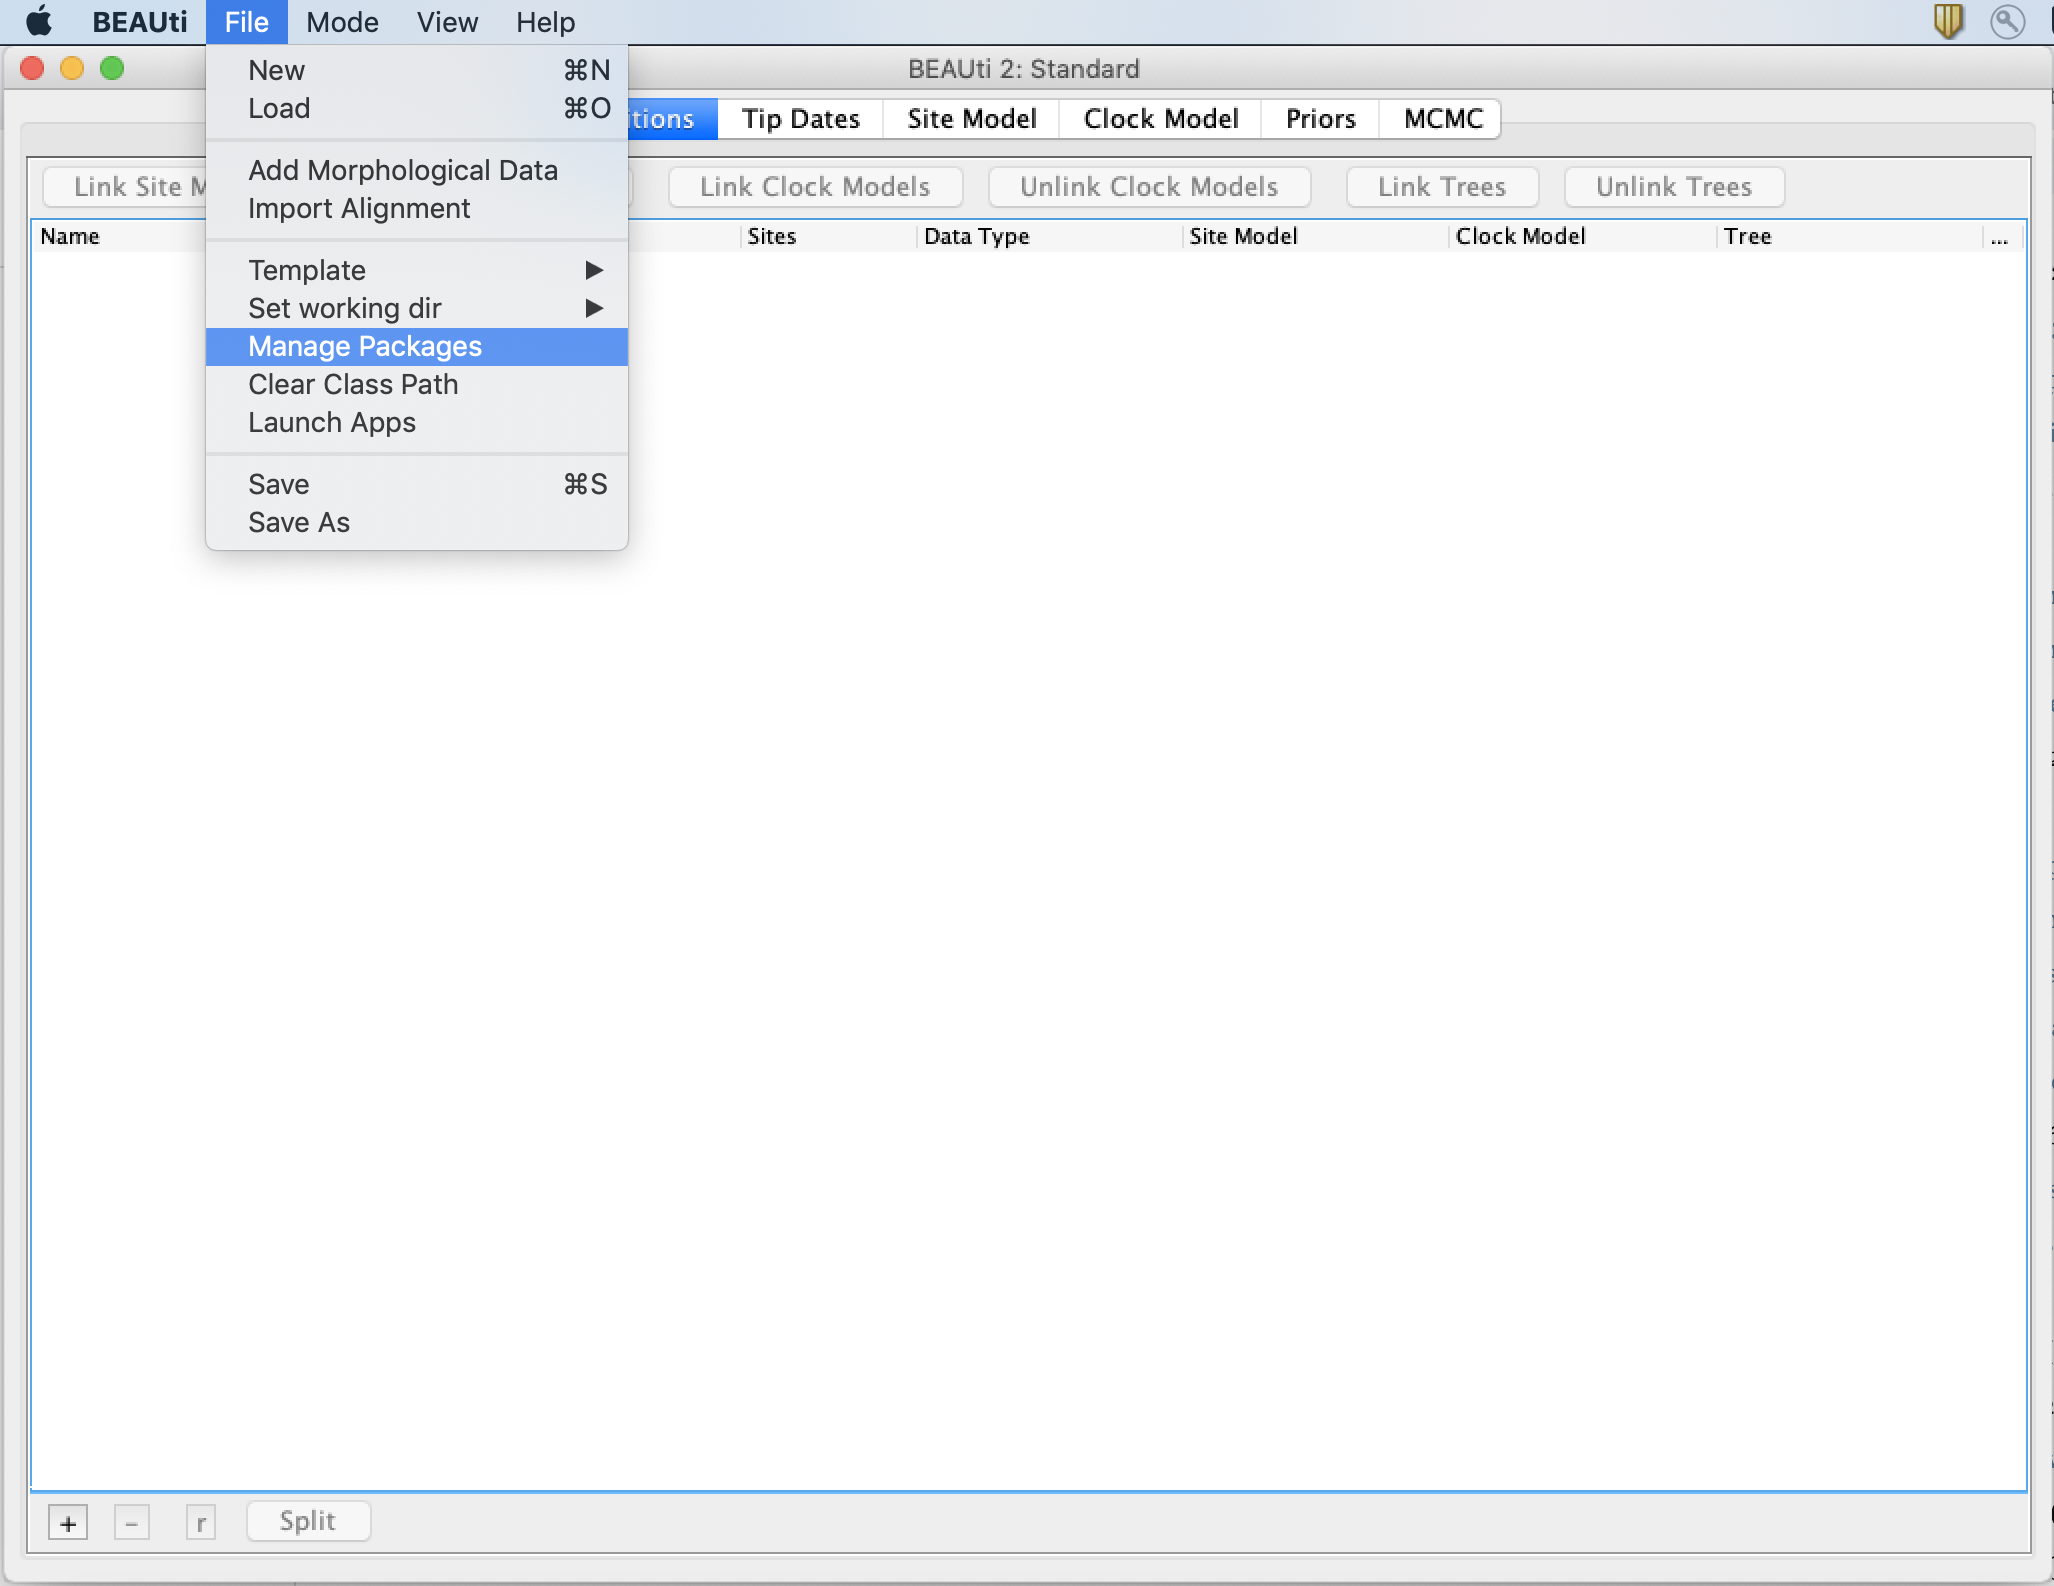
\includegraphics[width=0.750000\textwidth]{figures/package_manager.png}
    \caption{Finding the BEAST2 Package Manager.}
    \label{packageManage1}
\end{figure}

\begin{framed}
Install the \textbf{MSBD} package by selecting it and clicking the
\textbf{Install/Upgrade} button. (Figure \ref{packageManage2})
\end{framed}

\begin{figure}
    \centering
    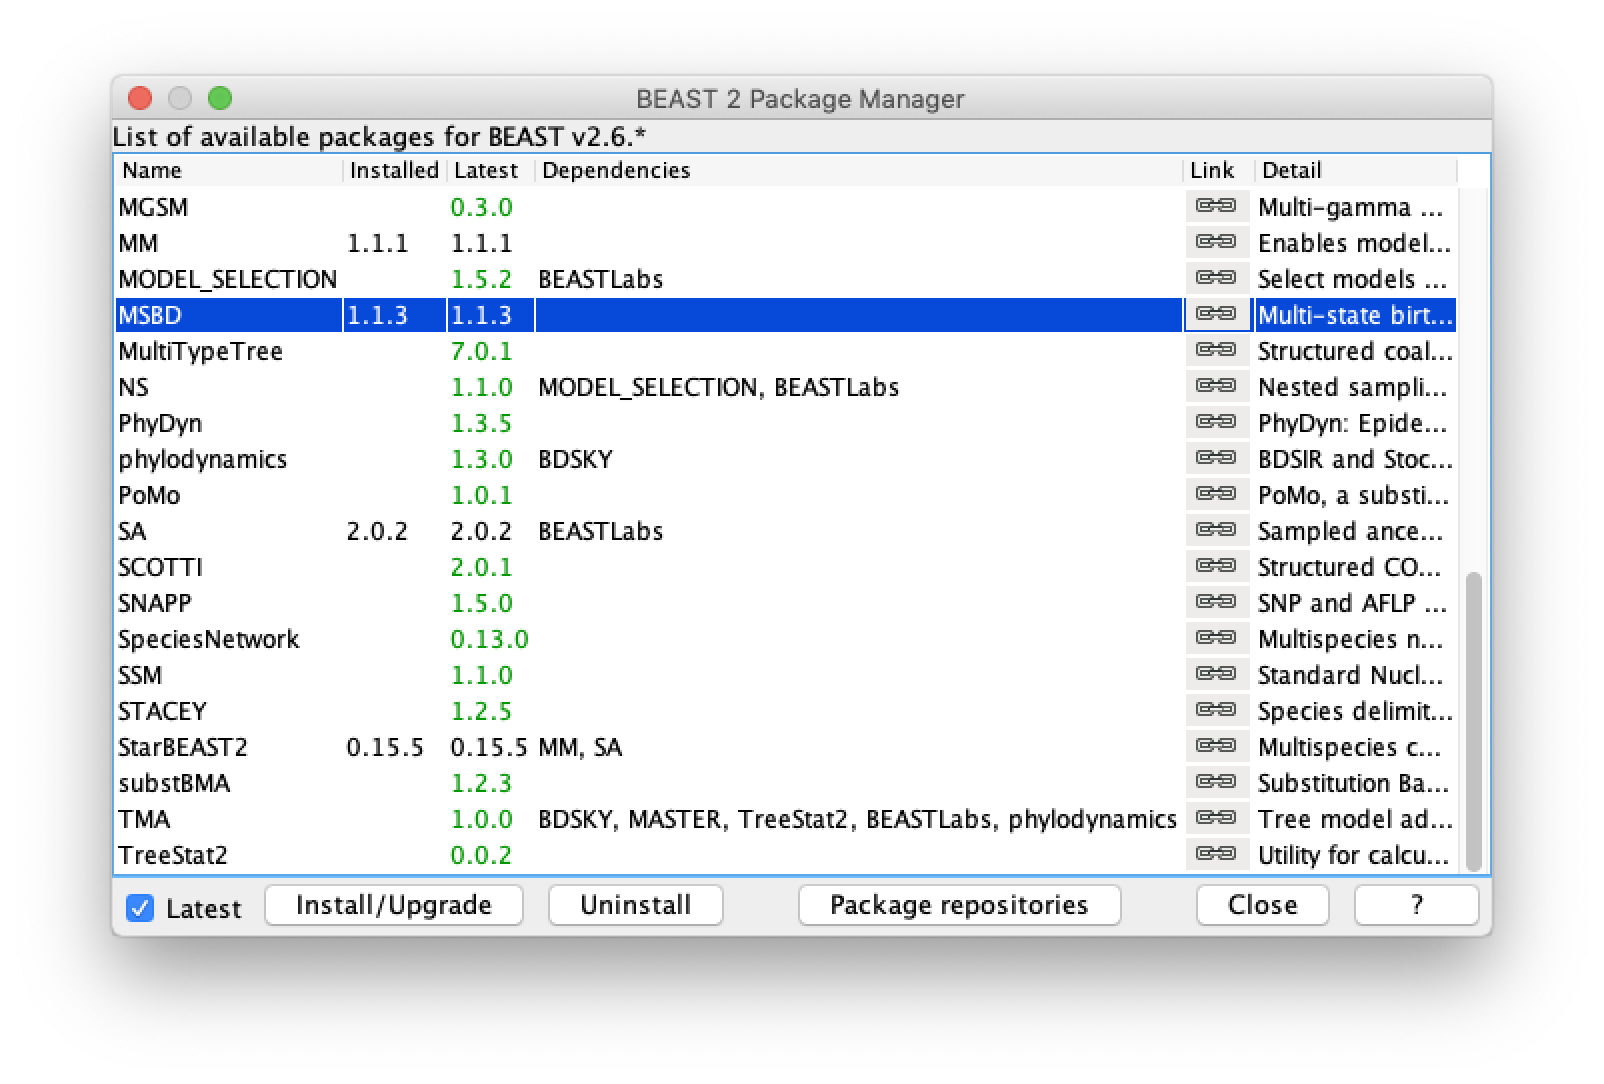
\includegraphics[width=0.650000\textwidth]{figures/packageMSBD.png}
    \caption{The BEAST2 Package Manager.}
    \label{packageManage2}
\end{figure}

BEAUti needs to be restarted for the newly installed package to be
loaded properly.

\begin{framed}
Close the \textbf{BEAST2 Package Manager} and \textbf{\emph{restart}}
BEAUti to fully load the \textbf{MSBD} package.
\end{framed}

\subsubsection{Setting the templates}\label{setting-the-templates}

BEAUti uses templates to define specific model configurations. The MSBD
template needs to be selected to set up an analysis using the MSBD
model.

\begin{framed}
Select the \textbf{MSBD template} by navigating to \textbf{File
\textgreater{} Template}. (Figure \ref{template})
\end{framed}

\begin{figure}
    \centering
    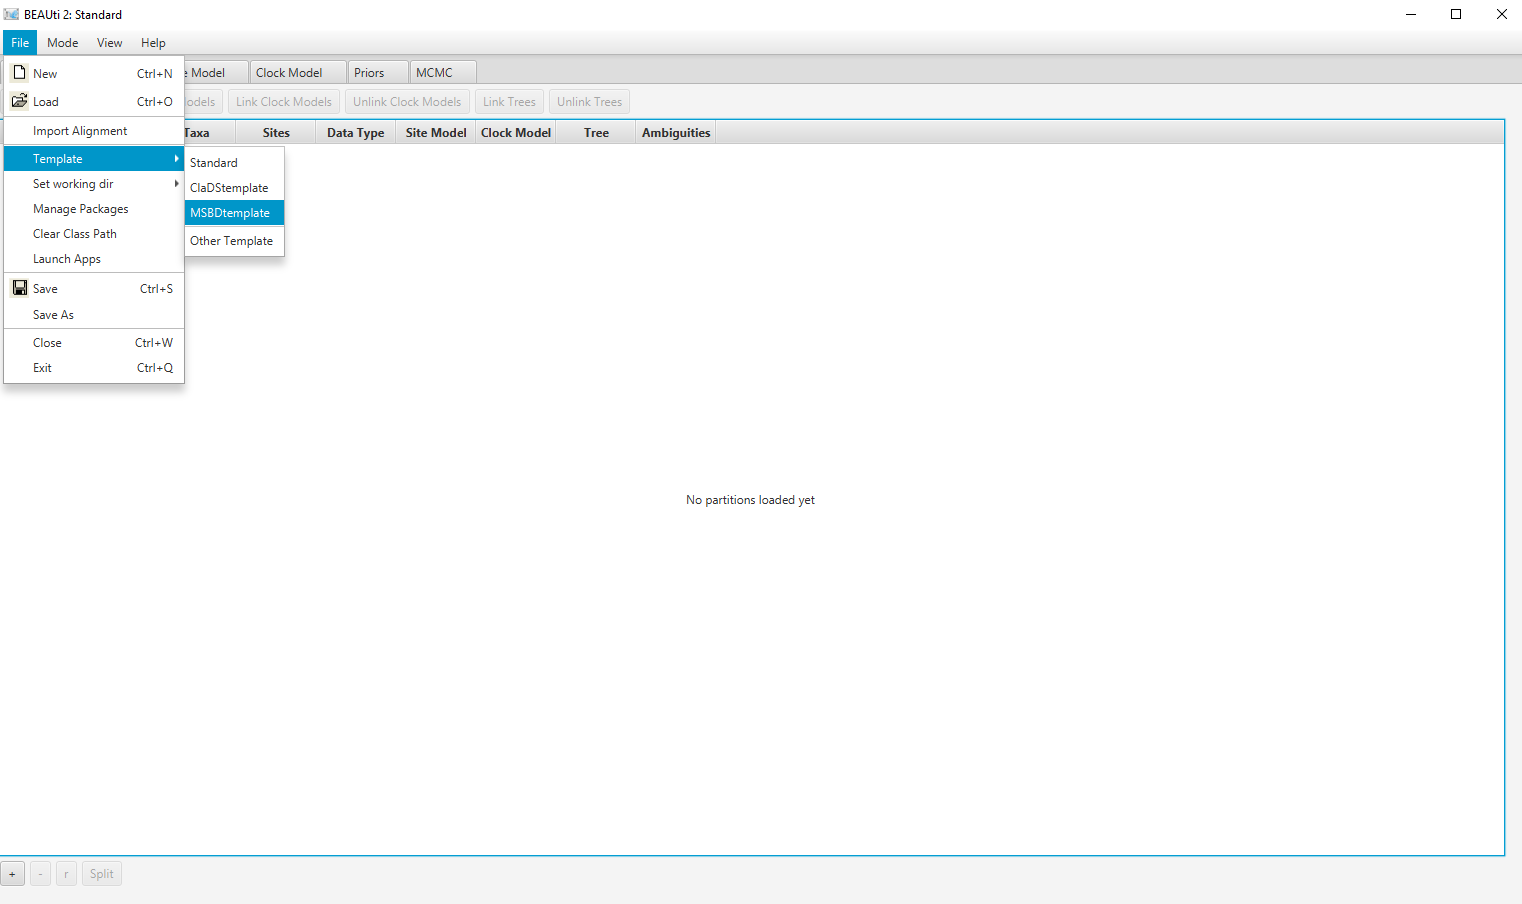
\includegraphics[width=0.750000\textwidth]{figures/template.png}
    \caption{Selecting the MSBD template.}
    \label{template}
\end{figure}

\subsubsection{Importing the alignment}\label{importing-the-alignment}

This analysis will be run with a fixed tree topology, however BEAUti
requires an alignment to be loaded in order to set the other components
of the model. As a result, we will load a dummy alignment, which is just
the sequence ``A'' for all taxa.

\begin{framed}
In the \textbf{Partitions} panel, import the alignment by navigating to
\textbf{File \textgreater{} Import Alignment} in the menu (Figure
\ref{importAlignment}) and then finding the \lstinline!hummingbirds.nex!
file on your computer \textbf{or} simply drag and drop the file into the
\textbf{BEAUti} window.
\end{framed}

\begin{figure}
    \centering
    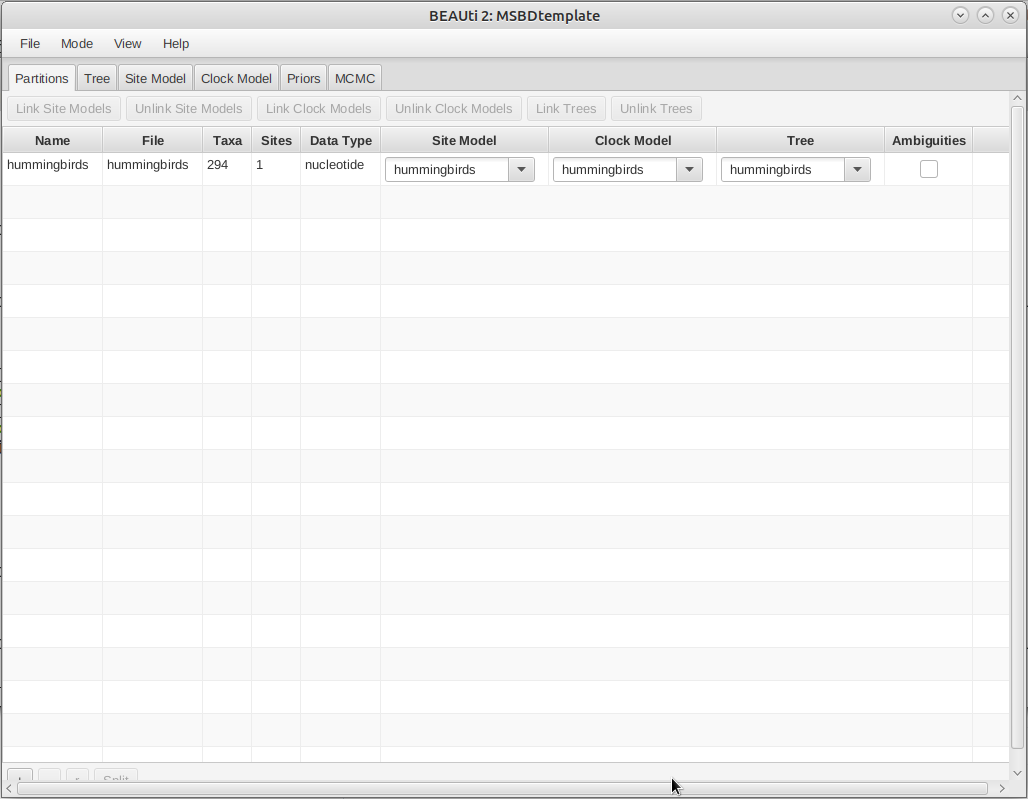
\includegraphics[width=0.750000\textwidth]{figures/alignment.png}
    \caption{Importing the alignment into BEAUti.}
    \label{importAlignment}
\end{figure}

\subsubsection{Importing the tree}\label{importing-the-tree}

As mentioned earlier, we want to run this analysis with a fixed tree
topology. By default BEAUti generates a random starting tree compatible
with the alignment, so we need to change this to our fixed tree.

\begin{framed}
In the \textbf{Tree} panel, set the dropdown to \textbf{Tree From
Newick}. Copy-paste the Newick tree found in the
\lstinline!hummingbirds.MCC.tre! file into the \textbf{Newick} field.
Uncheck the \textbf{Estimate Topology} checkbox.
\end{framed}

The final tree configuration is shown in Figure \ref{importTree}.

\begin{figure}
    \centering
    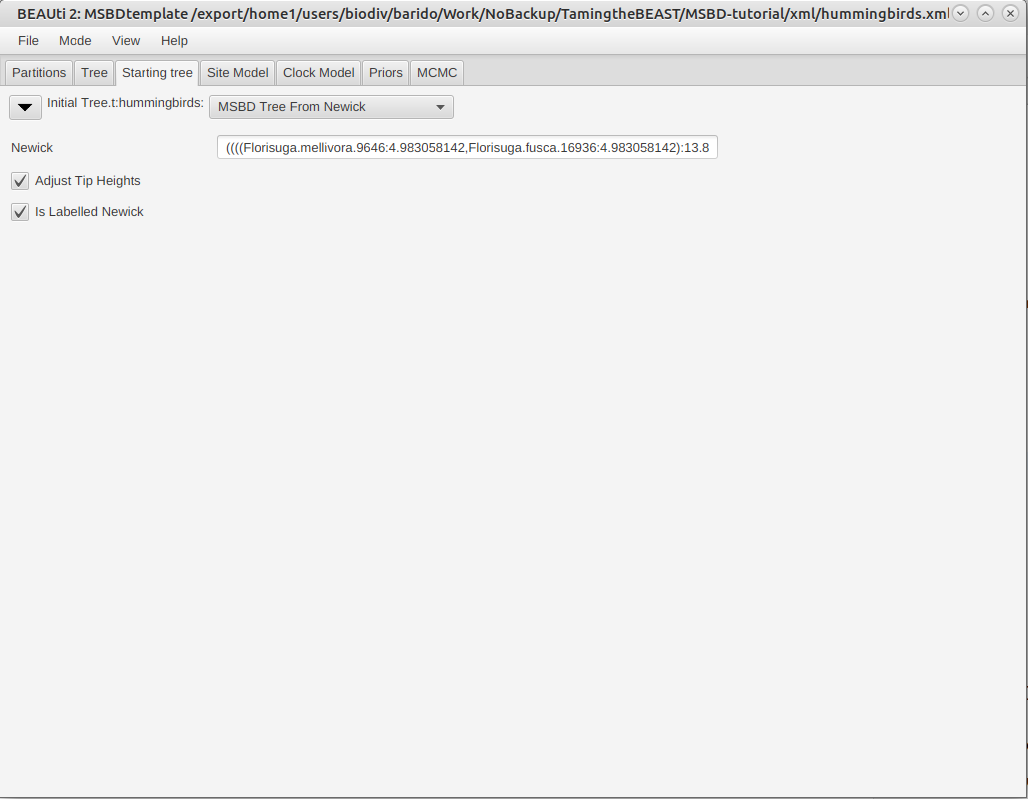
\includegraphics[width=0.750000\textwidth]{figures/tree.png}
    \caption{Importing the tree into BEAUti.}
    \label{importTree}
\end{figure}

\subsubsection{The parameter priors}\label{the-parameter-priors}

The next step is to look at the parameter priors, in the \textbf{Priors}
panel. The default priors on the birth rates
($ \lambda_i $), death rates ($ \mu_i $) and
total number of types ($ n_* $) are reasonable for this
dataset so we will not change them.

The expected average number of type changes across the entire tree is
given by $ n = \gamma \times L $, where L is the total
length of the tree. The length of the fixed tree used in this analysis
is $ \approx 1482 $, so the default prior on
$ \gamma $ would lead to a high expected number of type
changes. From the previous analysis performed in BAMM, we expect only a
few type changes across this phylogeny, so we will set the prior on
$ \gamma $ to a lower range, using a \textbf{LogNormal(-4.0,
1.0)} distribution.

\begin{framed}
Click on the arrow next to \textbf{gamma} and change the value for
\textbf{M} (mean) of the default log normal distribution to \textbf{-4}
(Figure \ref{gammaPrior}).
\end{framed}

\begin{figure}
    \centering
    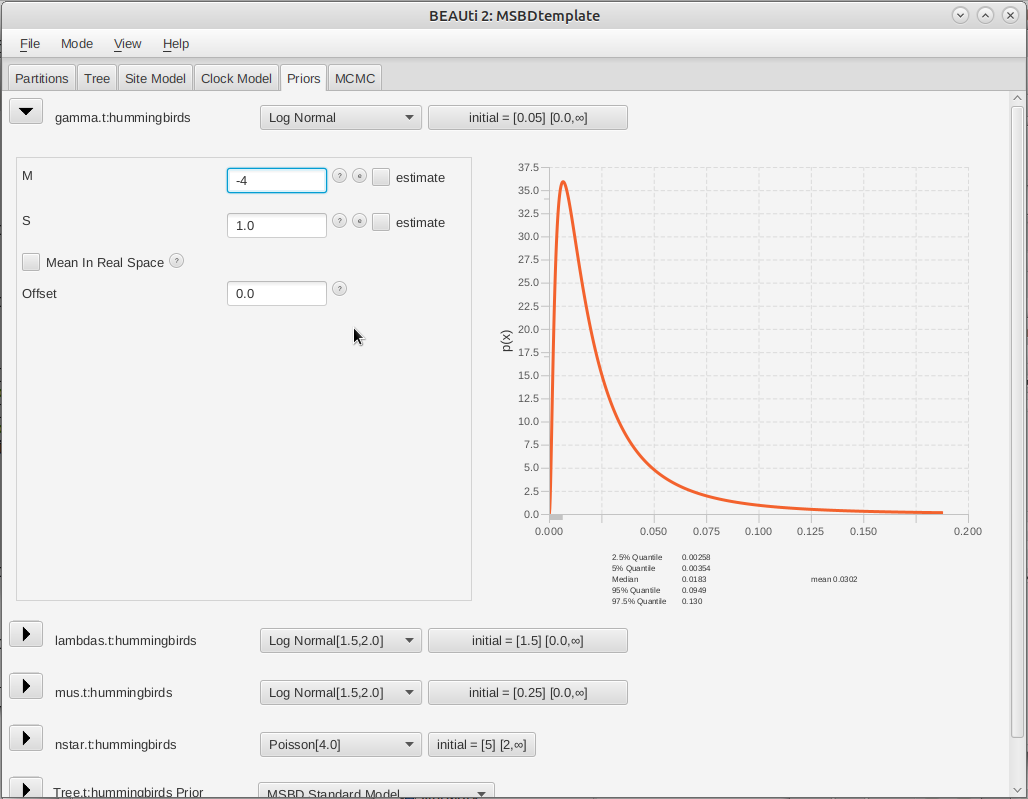
\includegraphics[width=0.750000\textwidth]{figures/gammaprior.png}
    \caption{Setting the prior on the type change rate.}
    \label{gammaPrior}
\end{figure}

\subsubsection{The tree prior}\label{the-tree-prior}

Next, we will specify the tree prior, i.e.~the MSBD model. By default
most of the parameters of the model are estimated, so it is not
necessary to change their starting values. However, the extant sampling
proportion ($ \rho $) and extinct sampling probability
($ \sigma $) are fixed. There are no extinct samples in this
dataset, and we have sampled 86\% of the extant hummingbirds species so
we will set $ \sigma = 0 $ and $ \rho = 0.86 $.

\begin{framed}
Click on the arrow next to \textbf{Tree} and change the value for
\textbf{rho} (extant sampling proportion) of the MSBD model to
\textbf{0.86} (Figure \ref{treePrior}).
\end{framed}

\begin{figure}
    \centering
    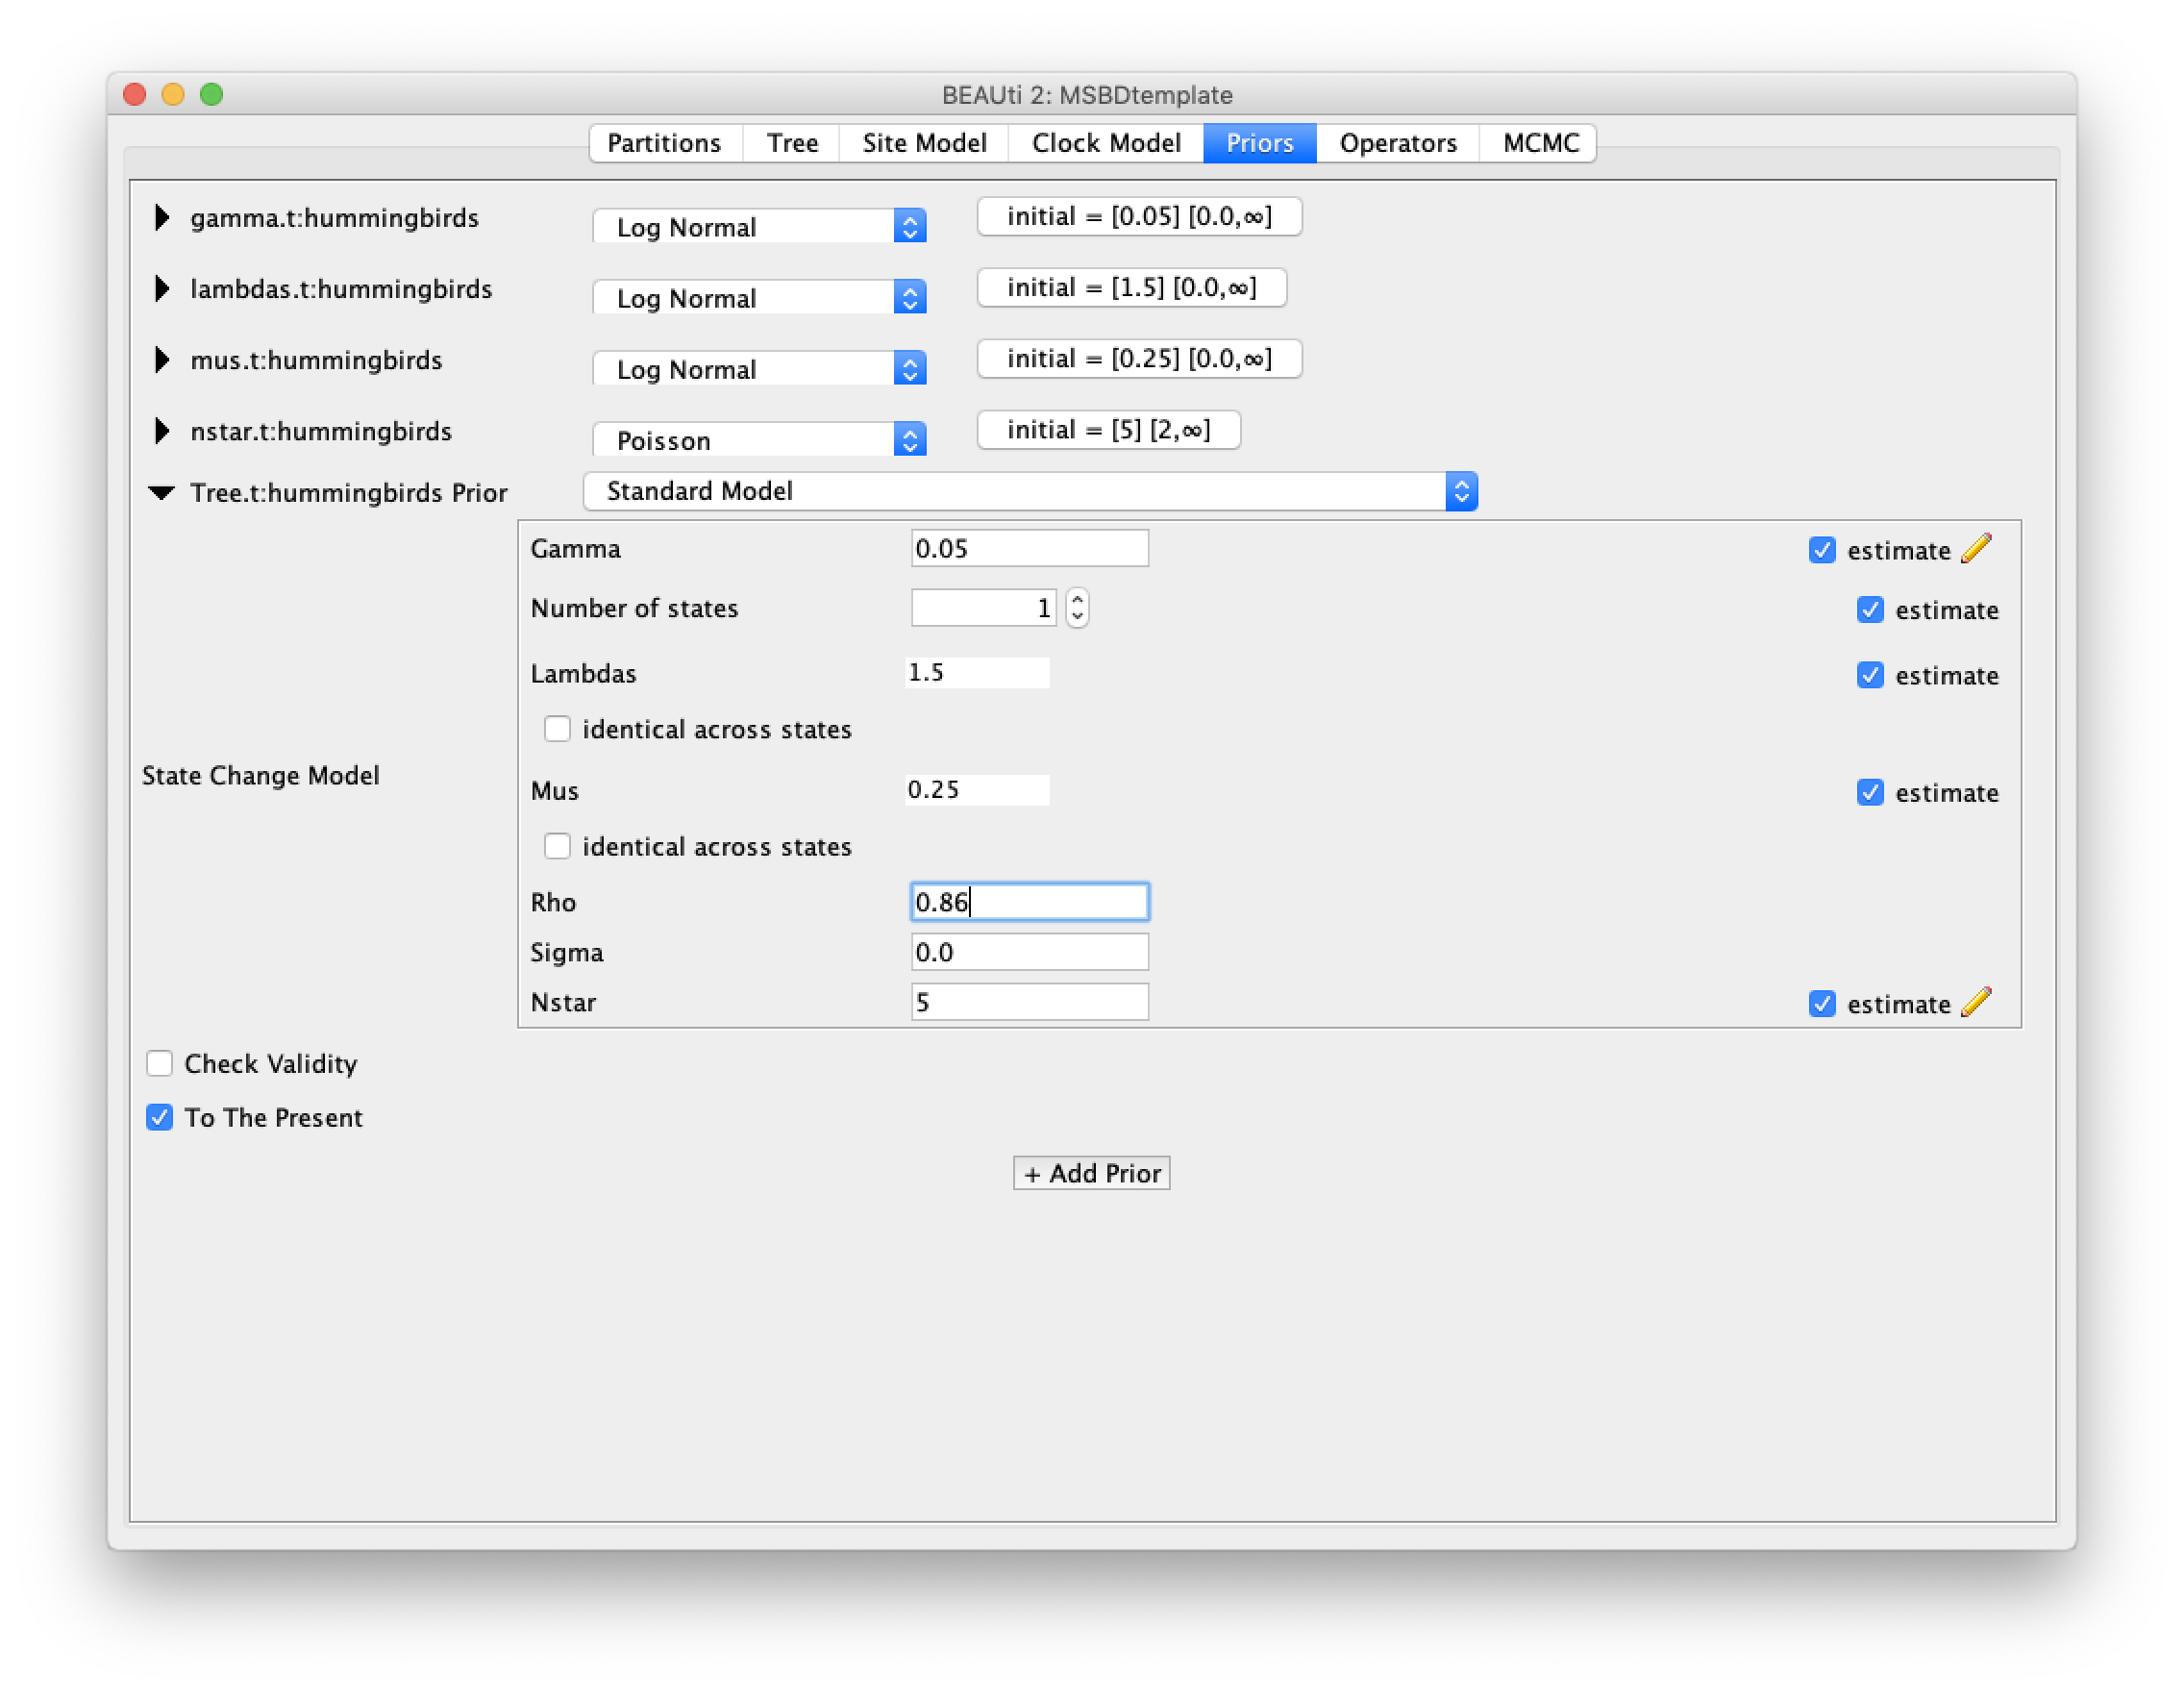
\includegraphics[width=0.750000\textwidth]{figures/treeprior.png}
    \caption{Setting the MSBD tree prior.}
    \label{treePrior}
\end{figure}

Note that many other options are available in this section, such as
fixing the number of states or the value of some parameters
(\textbf{estimate} checkboxes), setting the birth rate or the death rate
to be shared between states (\textbf{identical across states}
checkboxes), or setting the model to only use sampling-through-time
(\textbf{To The Present} checkbox) .

\subsubsection{MCMC options}\label{mcmc-options}

The next step is to set the options for running the chain, in the
\textbf{MCMC} panel. We can see that several loggers are set by default:

\begin{itemize}

\item
  the regular trace log, which in our case only records the posterior,
  likelihood and prior, as we are not using a substitution or clock
  model.
\item
  the screenlog, which shows the advancement of the chain to the screen.
\item
  the tree log, which will log the trees in Nexus format, with the birth
  and death rate on each edge as metadata.
\item
  the state change model log, which logs the parameters associated with
  the model, i.e. $ \gamma $, $ n_* $, the
  number of sampled states and the birth and death rates for each state
  ($ \lambda_i $ and $ \mu_i $).
\item
  the tip rates log, which logs the birth and death rates at each tip
  (optionally, at each node if the \textbf{nodeLog} option is
  activated).
\end{itemize}

These last three logs are specific to MSBD. The only thing we will
change here is the number of states recorded in the model. By default,
only the sampled states are recorded, however this results in a log that
is not in table format and so cannot be easily loaded into Tracer.
Fixing the number of recorded states solves this problem.

\begin{framed}
In the \textbf{MCMC} panel, click on the arrow next to
\textbf{stdStateslog} and click on the \textbf{Edit} button to the right
of the \textbf{StateChangeModelLogger} (Figure \ref{logs}).
\end{framed}

\begin{figure}
    \centering
    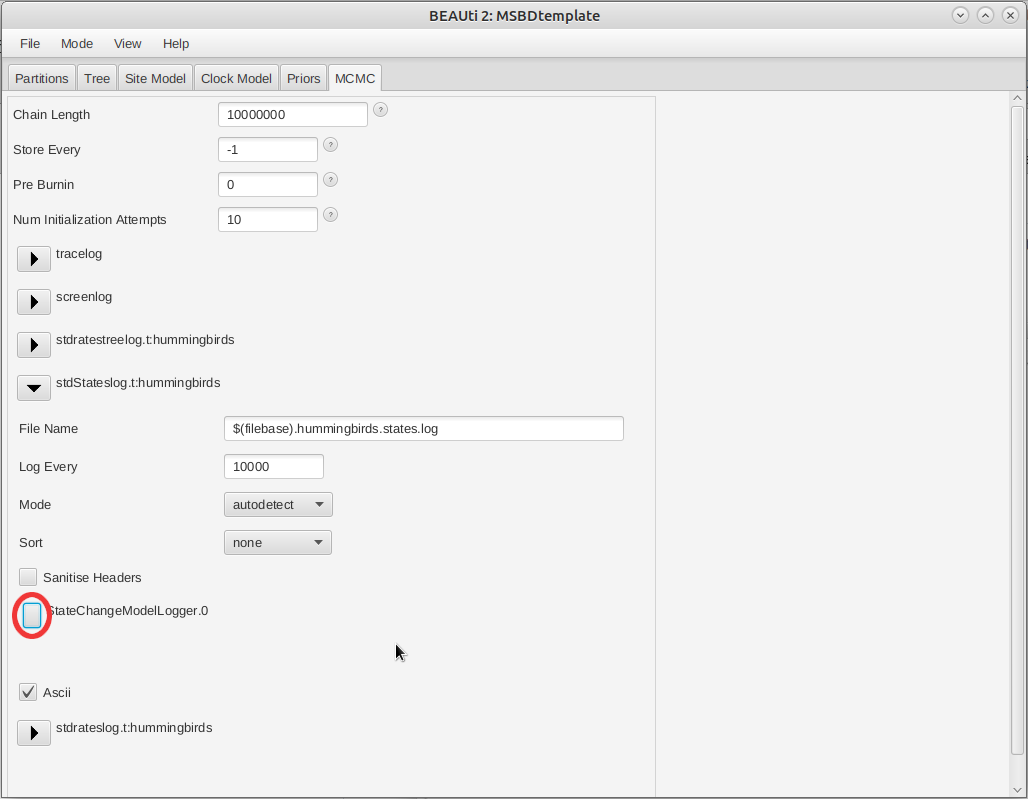
\includegraphics[width=0.750000\textwidth]{figures/logs.png}
    \caption{Opening the state change model log.}
    \label{logs}
\end{figure}

\begin{framed}
In the new panel, set the value of \textbf{maxStates} to 10 (Figure
\ref{logpanel}). Close the panel by clicking on \textbf{OK}.
\end{framed}

\begin{figure}
    \centering
    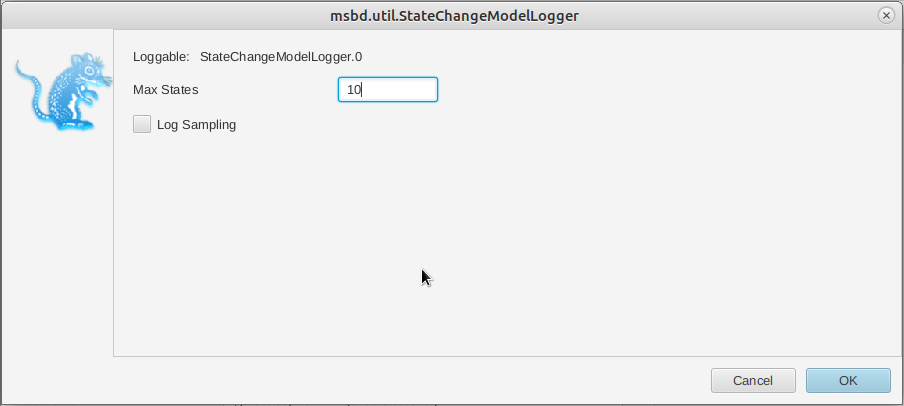
\includegraphics[width=0.650000\textwidth]{figures/logstates.png}
    \caption{Setting the state change model log.}
    \label{logpanel}
\end{figure}

Once all the options have been set, the final step is to save the XML.

\begin{framed}
Save the XML file as \lstinline!hummingbirds.xml! by navigating to
\textbf{File \textgreater{} Save}.
\end{framed}

\subsection{Running the analysis in
BEAST2}\label{running-the-analysis-in-beast2}

\begin{framed}
Start \textbf{BEAST2} and choose the file \lstinline!hummingbirds.xml!.

If you have \textbf{BEAGLE} installed tick the box to \textbf{Use BEAGLE
library if available}, which will make the run faster.

Hit \textbf{Run} to start the analysis.
\end{framed}

The run should take about 15-20 minutes.

\subsection{Analyzing the output}\label{analyzing-the-output}

\subsubsection{Output files}\label{output-files}

Our run has generated 4 different files:

\begin{itemize}

\item
  \lstinline!hummingbirds.log! which is the general trace log.
\item
  \lstinline!hummingbirds.hummingbirds.states.log! which recorded the
  parameters associated with the state model.
\item
  \lstinline!hummingbirds.hummingbirds.rates.log! which recorded the
  rates on tips of the tree.
\item
  \lstinline!hummingbirds.hummingbirds.rates.trees! which recorded the
  sampled trees in Nexus format.
\end{itemize}

\subsubsection{Analyzing the log files}\label{analyzing-the-log-files}

We will use the software Tracer to analyze the log files. The general
trace log is not very interesting in our case, as we used a fixed tree.
Next, we will look at the MSBD model log, contained in the file
\lstinline!hummingbirds.hummingbirds.states.log!. Figure \ref{gamma}
shows the estimated posterior distribution for the type change rate,
which in this analysis has a median estimate of 5.35E-3, with a 95\% HPD
of {[}4.04E-4 ; 0.014{]}.

\begin{figure}
    \centering
    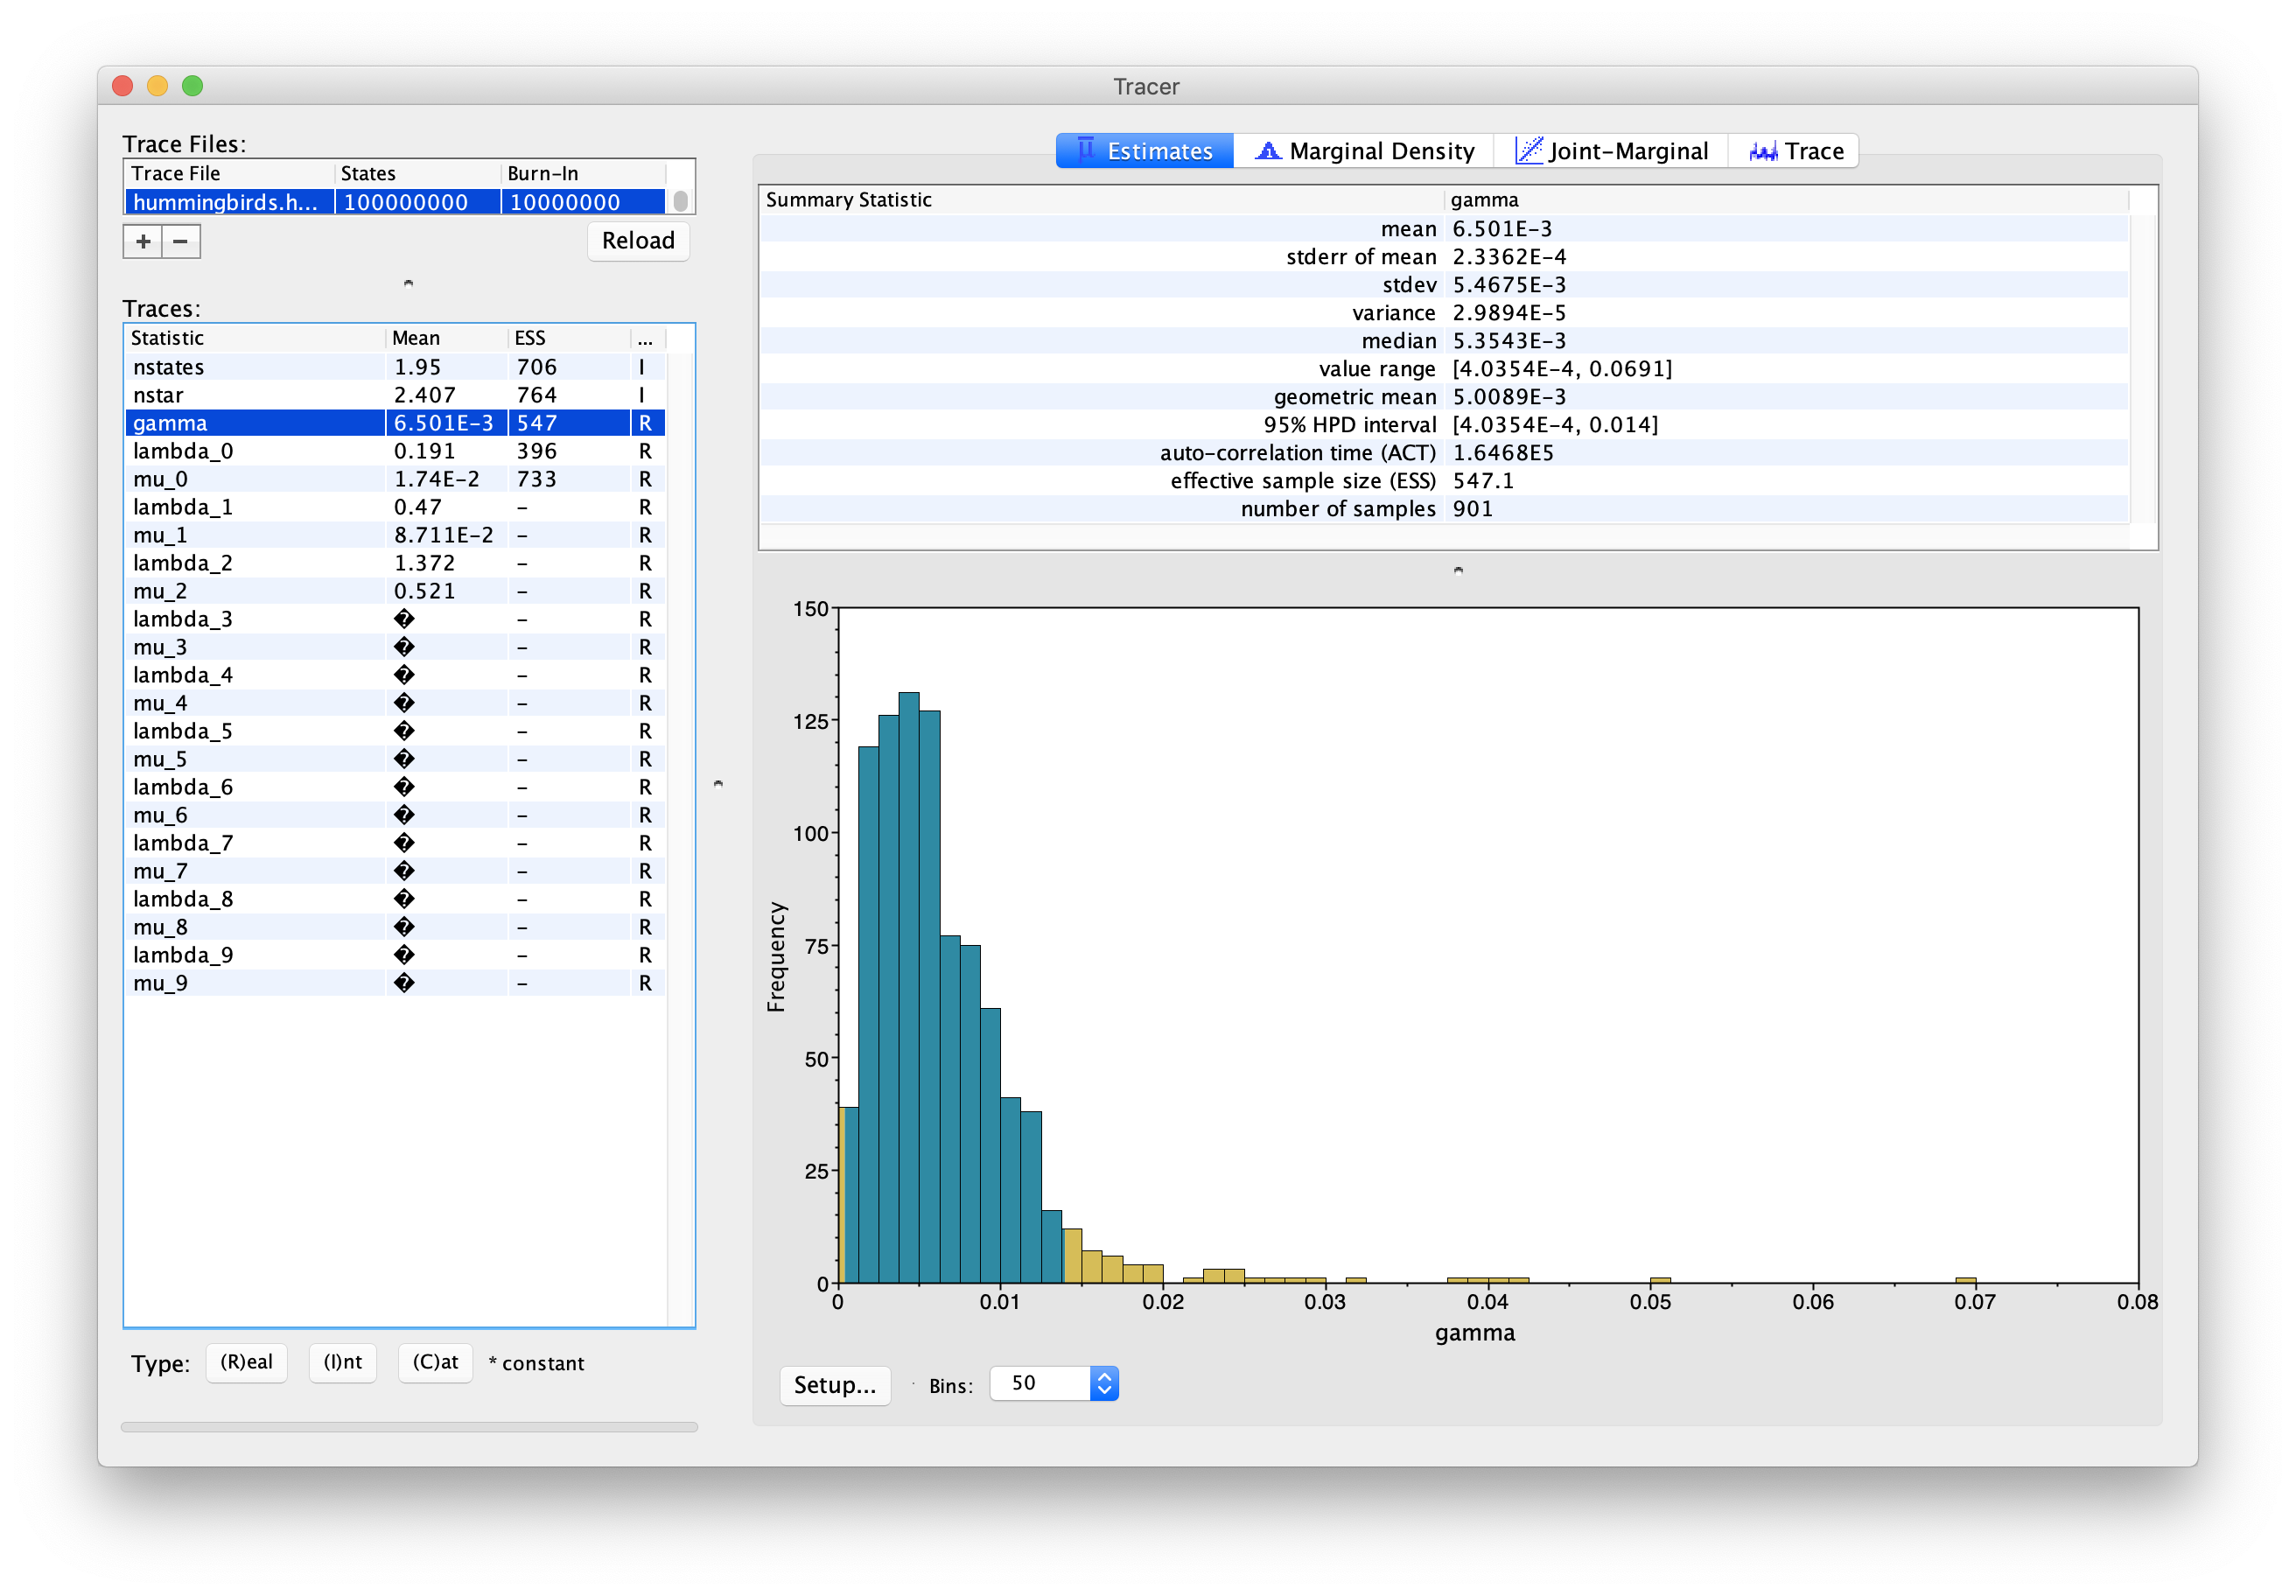
\includegraphics[max width=\textwidth, max height=0.9\textheight]{figures/tracer_gamma.png}
    \caption{Estimated posterior distribution of the type change rate, as shown in Tracer.}
    \label{gamma}
\end{figure}

One important thing to note is that the estimates of \lstinline!lambda!
and \lstinline!mu! in this log should not be directly used. This is due
to the fact that the types in our model are not tied to tips, so they
may not represent the same evolutionary regimes in all samples. For
instance, in the presence of two regimes, there may be samples where
type 0 corresponds to the regime with higher birth, while in other
samples this regime is represented by type 1. We can see this in Figure
\ref{lbda}, where the estimate for \lstinline!lambda_0! shows a
discrepancy around 6.5E7 samples, which corresponds to
\lstinline!lambda_0! and \lstinline!lambda_1! exchanging values. This
also means that ESS values for these parameters may be low even if the
chain has converged.

\begin{figure}
    \centering
    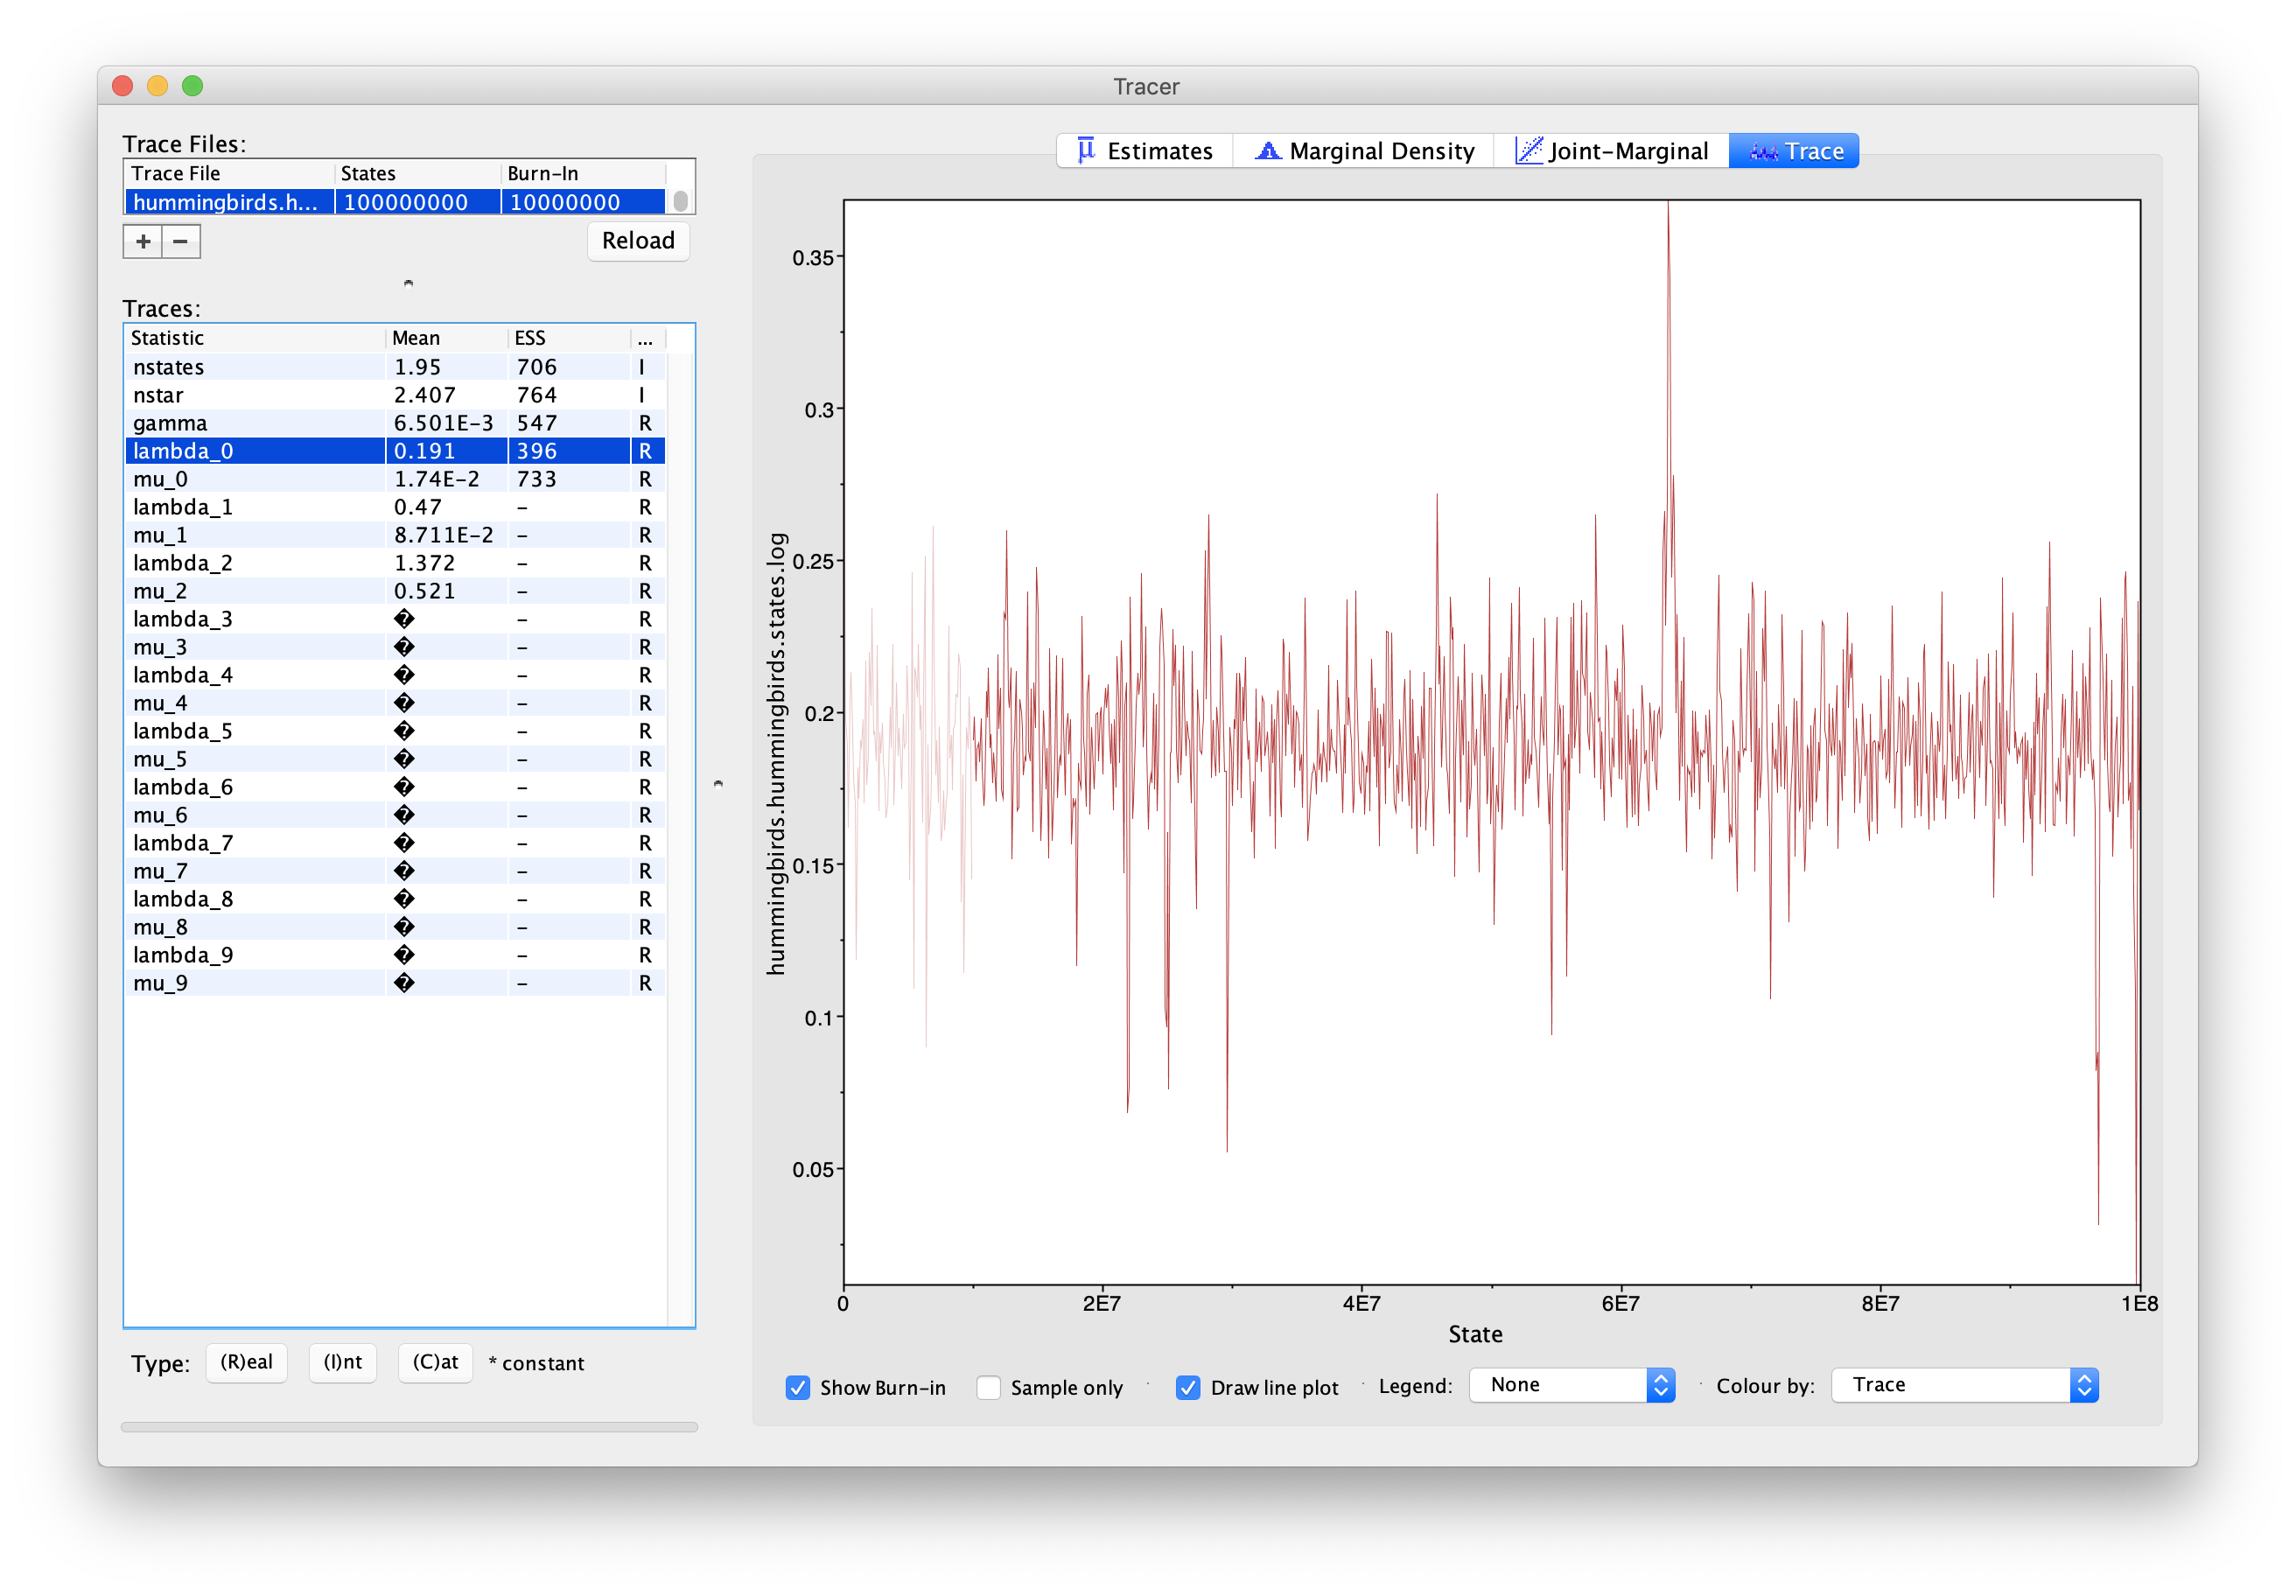
\includegraphics[max width=\textwidth, max height=0.9\textheight]{figures/tracer_lambda.png}
    \caption{Trace of the birth rate for type 0, as shown in Tracer.}
    \label{lbda}
\end{figure}

In order to look at the actual birth and death rates estimates, we can
look at the tip rates log, stored in the file
\lstinline!hummingbirds.hummingbirds.rates.log!. Figure \ref{tip_uni}
and Figure \ref{tip_bi} show examples of the estimated posterior
distributions of the birth rate for two different tips.

\begin{figure}
    \centering
    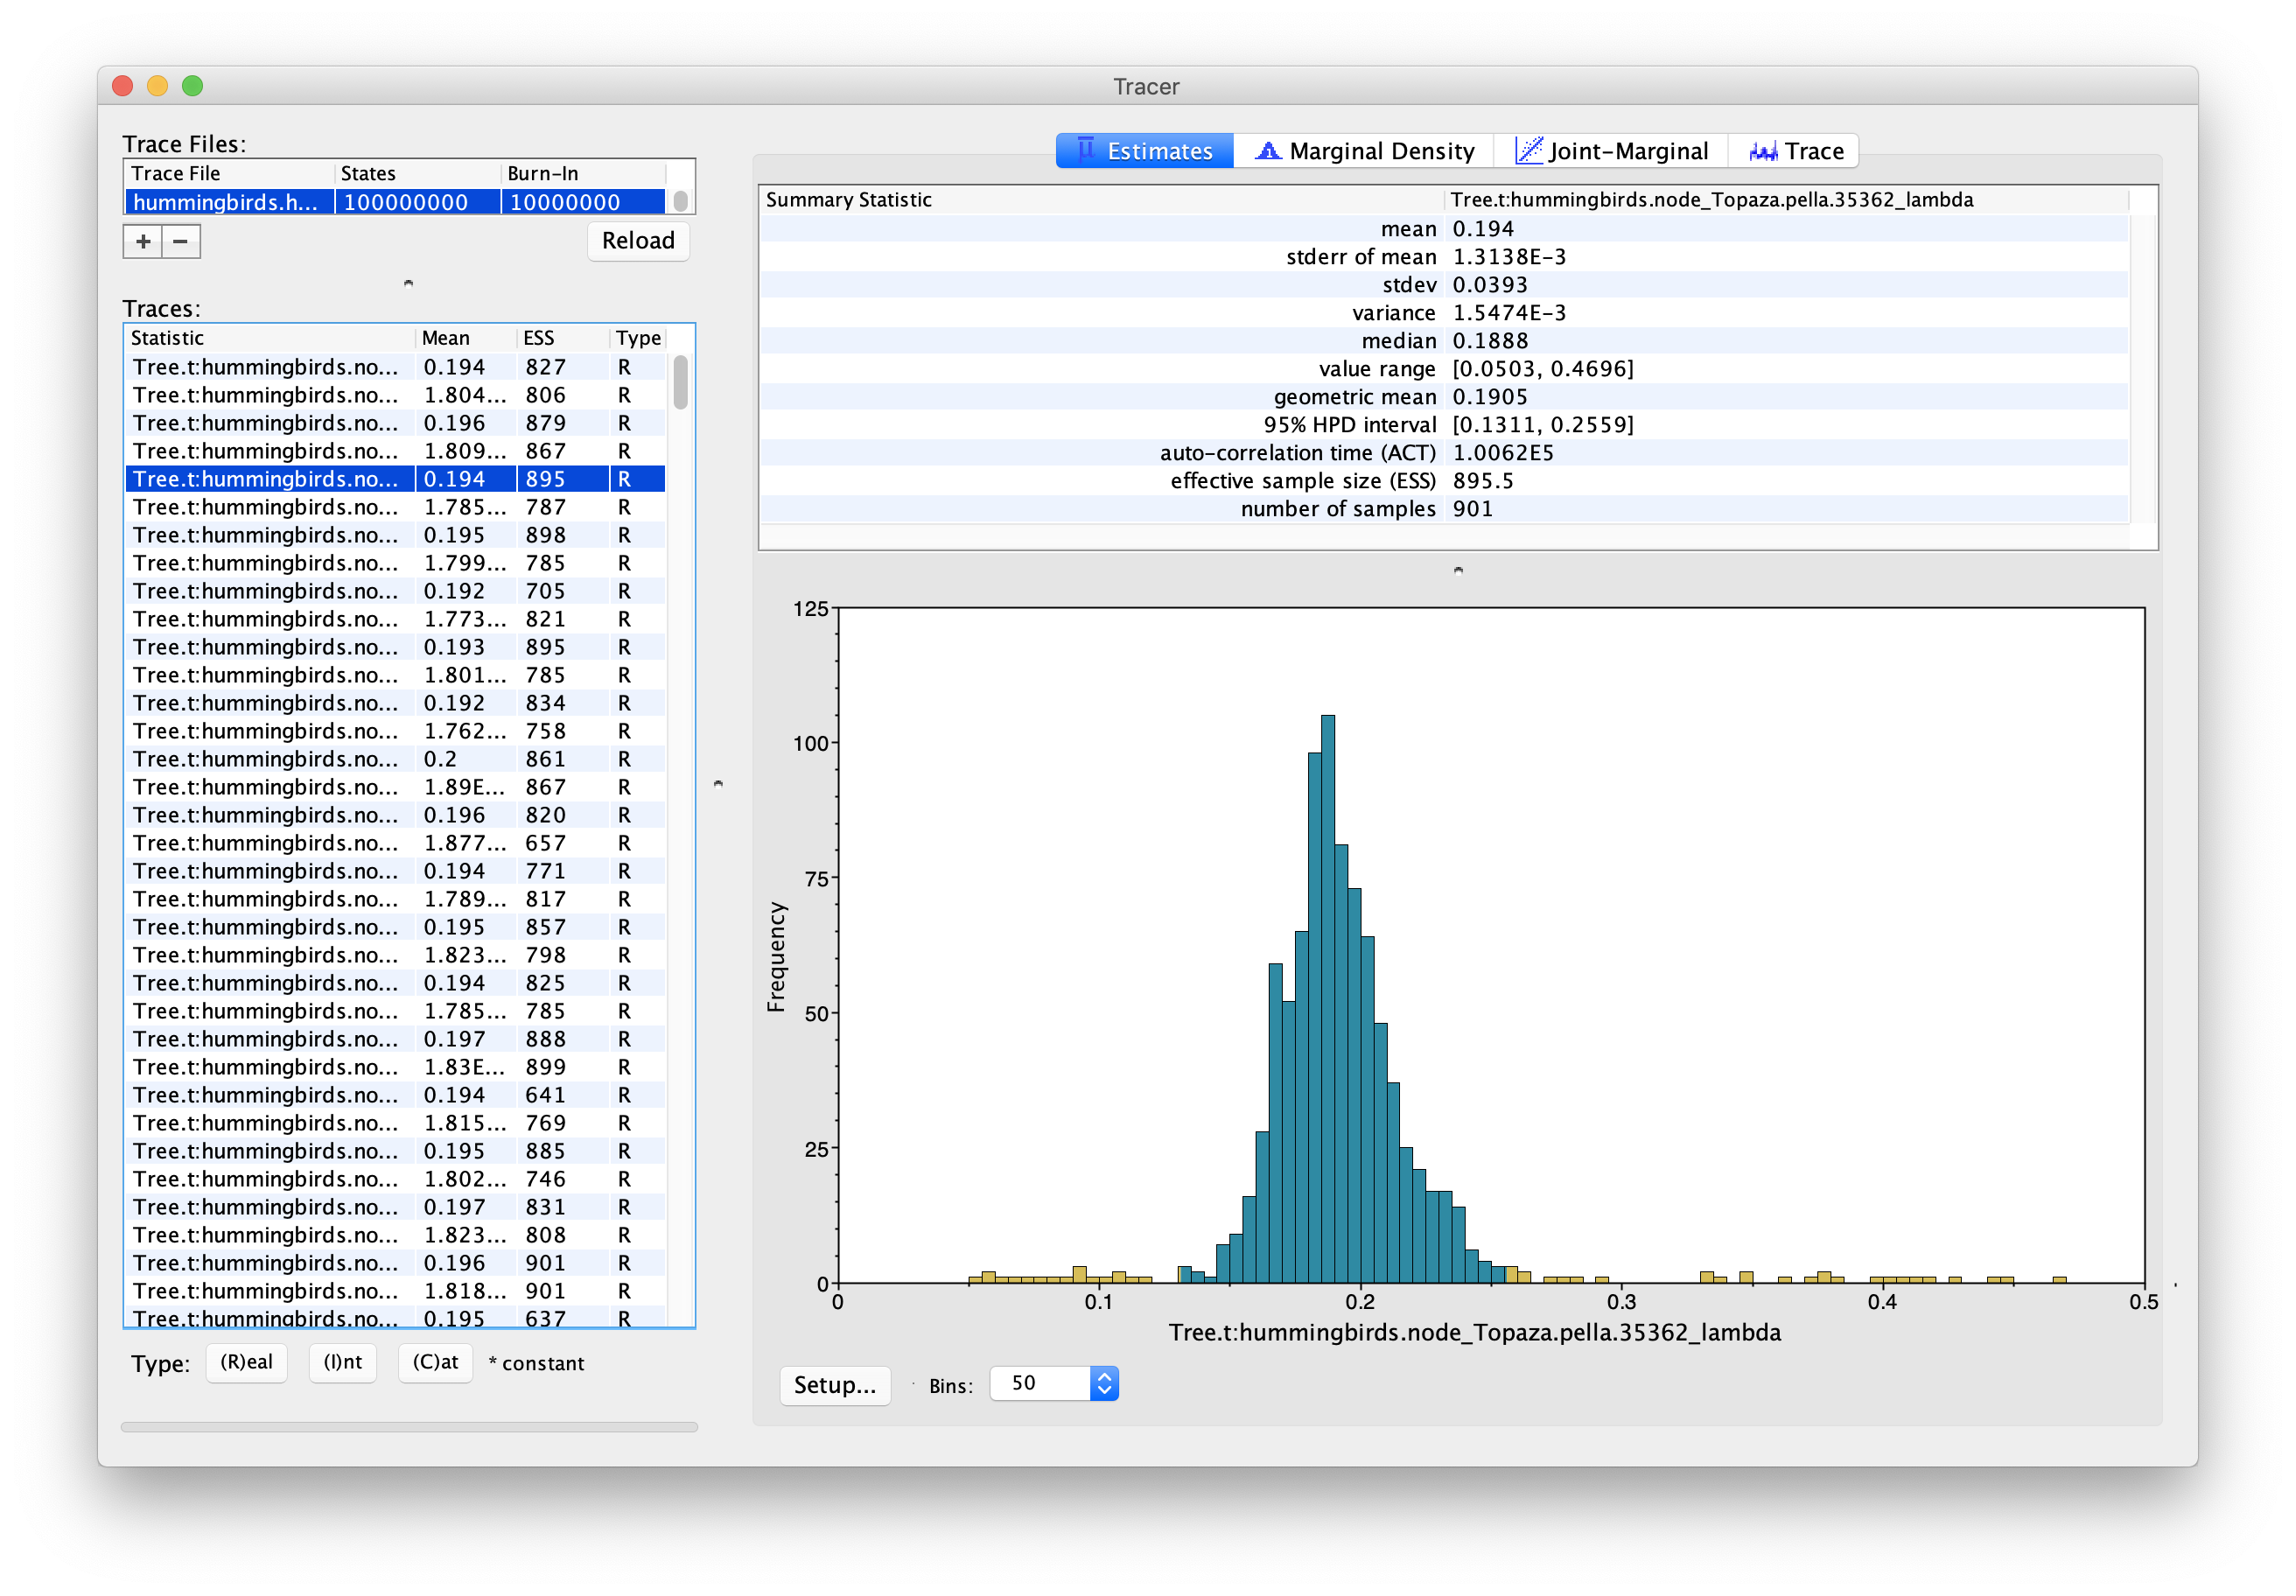
\includegraphics[max width=\textwidth, max height=0.9\textheight]{figures/tracer_tip_unim.png}
    \caption{Estimated posterior distribution of the birth rate at tip Topaza.pella, as shown in Tracer.}
    \label{tip_uni}
\end{figure}

\begin{figure}
    \centering
    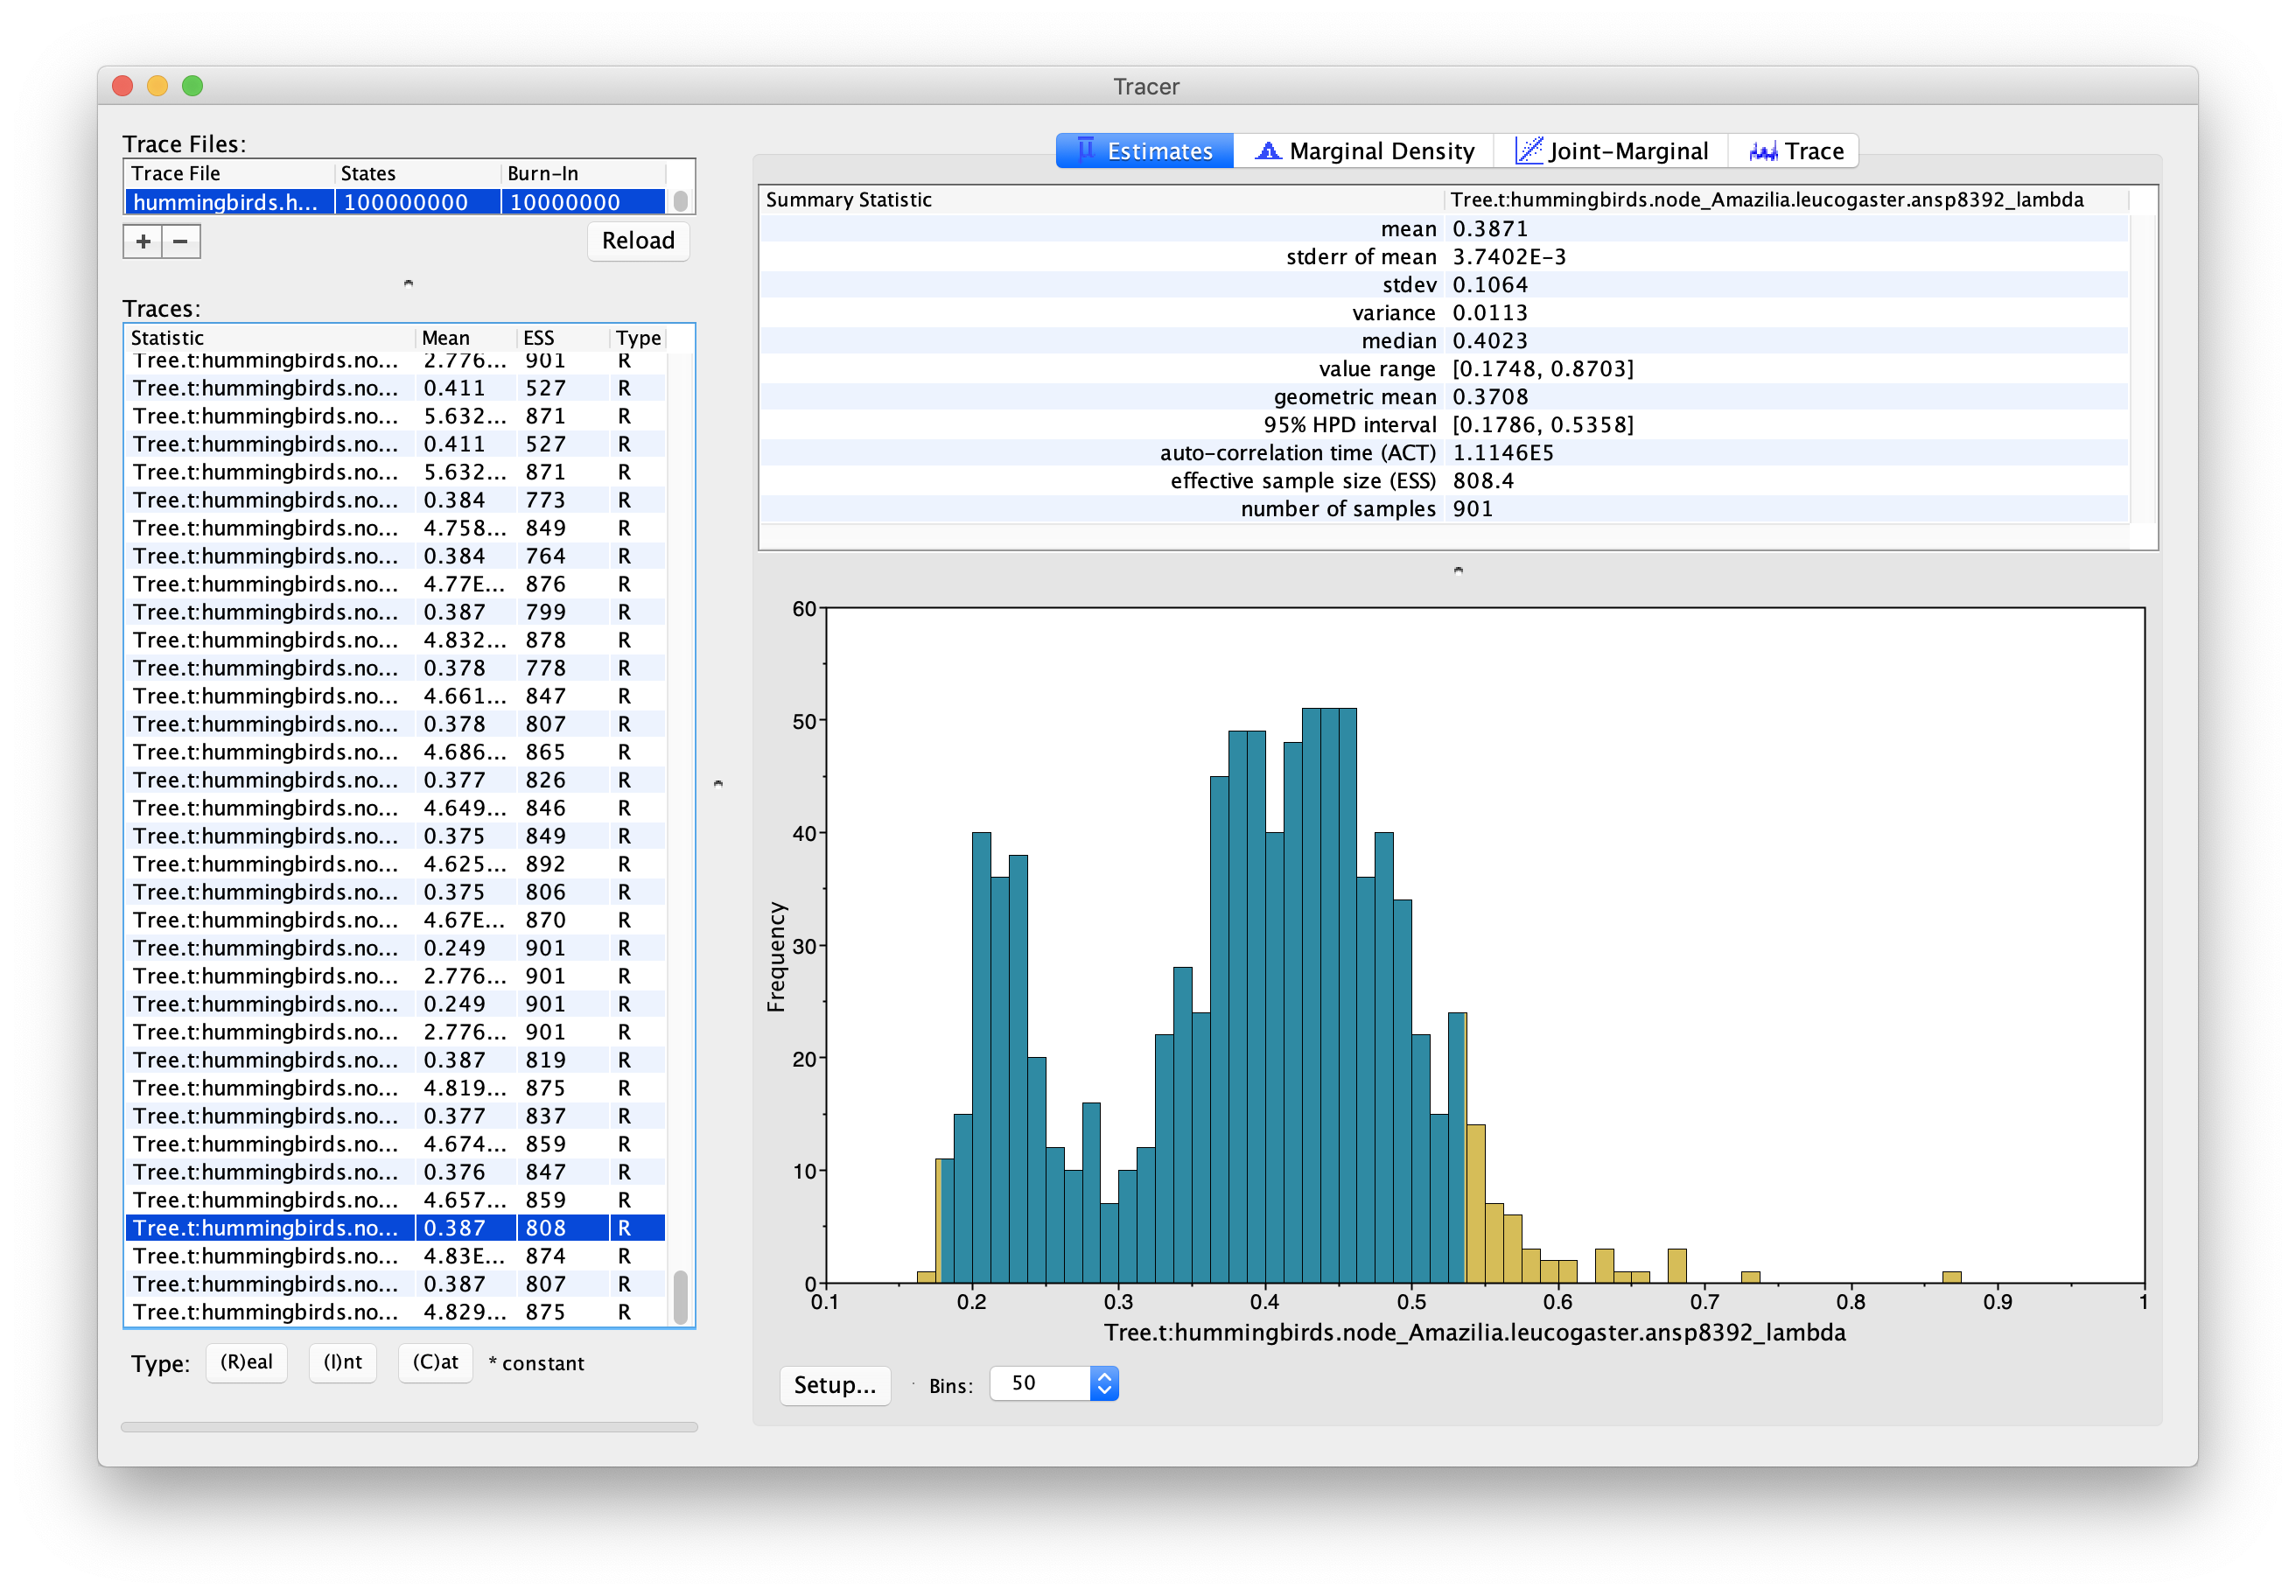
\includegraphics[max width=\textwidth, max height=0.9\textheight]{figures/tracer_tip_bim.png}
    \caption{Estimated posterior distribution of the birth rate at tip Amazilia.leucogaster, as shown in Tracer.}
    \label{tip_bi}
\end{figure}

We can see that these two tips present two very different
configurations. The first tip shows a unimodal posterior distribution,
which indicates that it is confidently assigned to one particular
evolutionary regime. On the other hand, the second tip presents a
bimodal distribution, indicating that there are two distinct
evolutionary regimes, with two distinct birth rates, which it can be
assigned to. This is important to note because the usual metrics used to
summarize posterior distributions, i.e.~the median and 95\% HPD
interval, work well in the first case but can give a misleading
representation of the posterior in the second case. In this case the
median estimate for the birth rate of \emph{Amazilia.leucogaster} is
0.40, which corresponds approximately to the second mode of the
distribution, however neither the median nor the 95\% HPD interval show
the existence of a second possible regime, with birth rate
$ \approx $0.22.

\subsubsection{Analyzing the trees}\label{analyzing-the-trees}

Another way to visualize the results is to look at the rates as plotted
on the tree. We can use TreeAnnotator to build an MCC tree from the tree
log in the file \lstinline!hummingbirds.hummingbirds.rates.trees!. Since
we also logged the birth and death rates for each edge in the tree log,
these parameters will also be summarized along with the tree.

\begin{framed}
Start \textbf{TreeAnnotator} and set the input tree to the tree log
file.

Set the burn-in percentage to 10\%.

Give a name to the output file, for instance
\lstinline!hummingbirds.MCC.tre!.

Finally, click \textbf{Run} to start the summary.
\end{framed}

The MCC tree can be loaded into any tree visualization software, such as
FigTree or IcyTree. We are going to use the R script provided in this
tutorial \lstinline!plot_MCC.R!. This script takes as input the MCC tree
file and an output file to store the plot, and it will plot the MCC tree
with edges coloured by the median estimates of the birth and death
rates. Run the following commands in an R console to create the plots:

\begin{lstlisting}[language=R]
source("plot_MCC.R")
MCC_colour_plot("hummingbirds.MCC.tre", plotfile = "hummingbirds_MCC.pdf")
\end{lstlisting}

Figure \ref{mcc_birth} and Figure \ref{mcc_death} show the resulting
plots for the birth rate and the death rate, respectively.

\begin{figure}
    \centering
    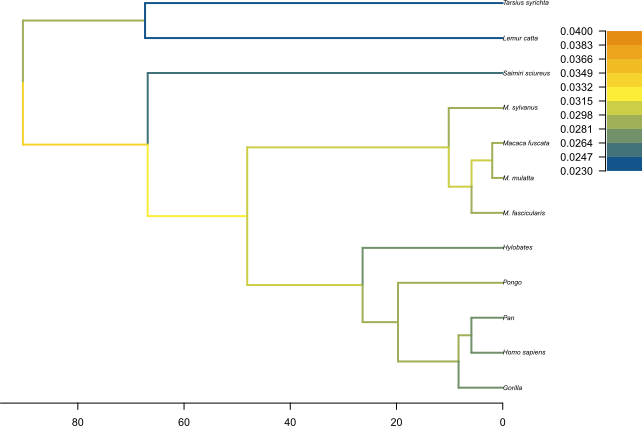
\includegraphics[max width=\textwidth, max height=0.9\textheight]{figures/mcc_birth.png}
    \caption{MCC tree with edges coloured by the median birth rate.}
    \label{mcc_birth}
\end{figure}

\begin{figure}
    \centering
    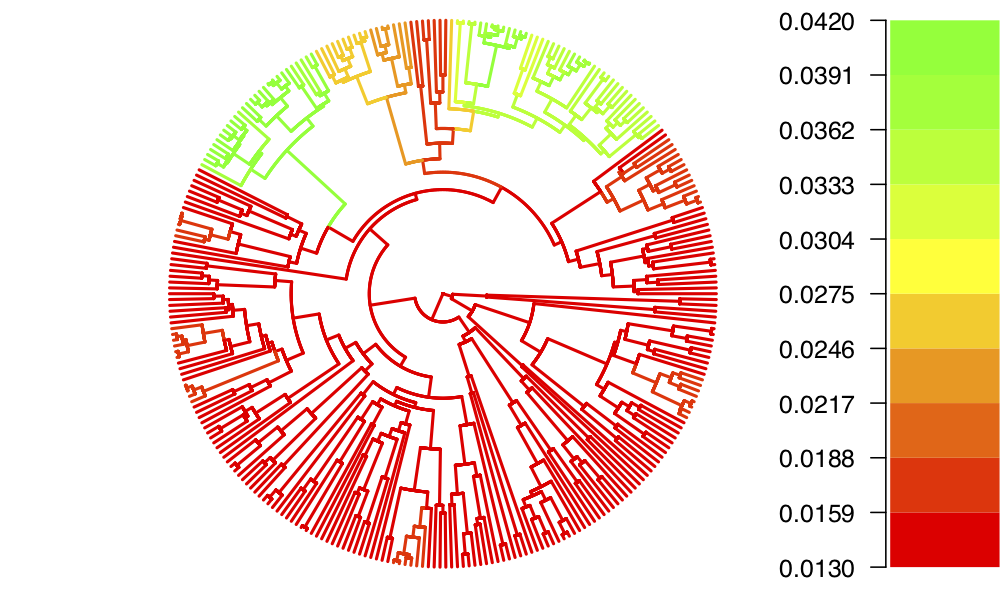
\includegraphics[max width=\textwidth, max height=0.9\textheight]{figures/mcc_death.png}
    \caption{MCC tree with edges coloured by the median death rate.}
    \label{mcc_death}
\end{figure}

We can see that while most of the tree shares one evolutionary regime
(in red), some clades are inferred to have evolved under a second regime
(in green), with higher birth and death rates. From this figure it is
not possible to tell whether the clades coloured in yellow-orange
represent a third intermediate regime, or whether there is uncertainty
as to which of the two regimes they belong to.

Going back to the rates log file and using the full posterior
distribution rather than just the median, we see that the intermediate
colour is likely due to uncertainty rather than a third regime.

\clearpage

\section{Useful Links}\label{useful-links}

\begin{itemize}

\item
  \href{http://www.beast2.org/book.html}{Bayesian Evolutionary Analysis
  with BEAST 2} \citep{BEAST2book2014}
\item
  BEAST 2 website and documentation: \url{http://www.beast2.org/}
\item
  BEAST 1 website and documentation: \url{http://beast.bio.ed.ac.uk}
\item
  Join the BEAST user discussion:
  \url{http://groups.google.com/group/beast-users}
\end{itemize}




%%%%%%%%%%%%%%%%%%%%%%%
% Tutorial disclaimer %
%%%%%%%%%%%%%%%%%%%%%%%
% Please do not change the license
% Add the author names and relevant links
% Add any other aknowledgments here
\href{http://creativecommons.org/licenses/by/4.0/}{
\includegraphics[scale=0.8]{figures/ccby.pdf}} This tutorial was written by Joëlle Barido-Sottani for \href{https://taming-the-beast.github.io}{Taming the BEAST} and is licensed under a \href{http://creativecommons.org/licenses/by/4.0/}{Creative Commons Attribution 4.0 International License}. 


%%%%%%%%%%%%%%%%%%%%
% Do NOT edit this %
%%%%%%%%%%%%%%%%%%%%
Version dated: \today


%%%%%%%%%%%%%%%%
%  REFERENCES  %
%%%%%%%%%%%%%%%%

\printbibliography[heading=relevref]


\end{document}